\begin{titlepage}
\begin{center}

\includegraphics[scale=0.15]{Documents/niser.png}
\line(1,0){300}\\
[2mm]
\begin{large}
\textbf{\huge Flip-Flop Circuits}\\ 
\end{large}
\line(1,0){150}\\
[5cm]
\large MAITREY SHARMA\\
\small (1911093)\\
[4.5cm]
Second Year Integrated M.Sc.\\
\textbf{School of Physical Sciences}\\
\textbf{National Institute of Science Education and Research, Bhubaneshwar}\\
\small March 24, 2021
\end{center} 
\end{titlepage}
\newpage
\section{Aim}
\noindent
To construct and study the operations of the following circuits:
\begin{enumerate}
    \item To construct half and full adder circuit and verify its working
    \item To construct half and full subtractor circuit and verify its working
    \item To construct a full adder-subtractor circuit
\end{enumerate}
\section{Apparatus}
\noindent Digital ICs 7402, 7408, 7400, 7404 and 7410, resistors, DC voltage source of $\SI{5}{\volt}$, LEDs, breadboard and connecting wires.
\section{Theory}
\noindent
\textbf{\emph{Combinational Logic Circuits}} are digital logical circuits whose output at any instant in time depends only on the combination of its inputs. That is, the output is determined by the logical function of their current input state, logic “0” or logic “1”, at any given instant in time. Any changes to the signals being applied to their inputs will immediately have an effect at the output, therefore, the output is dependant at all times on the combination of its inputs.
\par
\noindent
Though, in many instances, it is desirable to have the previous output playing a role in determining the current output. For relaying this information of the previous output, the circuit needs to have an \emph{memory} element. Technically speaking, a \textbf{\emph{memory}} is a device or system that is used to store information for immediate use in a computer or related computer hardware and digital electronic devices. The type of digital logical circuits that use memory elements so as to take account the previous and current states simultaneously are known as \textbf{\emph{Sequential Logic Circuits}}.
\par
\noindent
The concept of memory element is based on \emph{feedback}. That is, the output of the digital logic circuit is being fed back into the input. The example below is a simple realization of such feedback logic circuit.
\begin{center}
    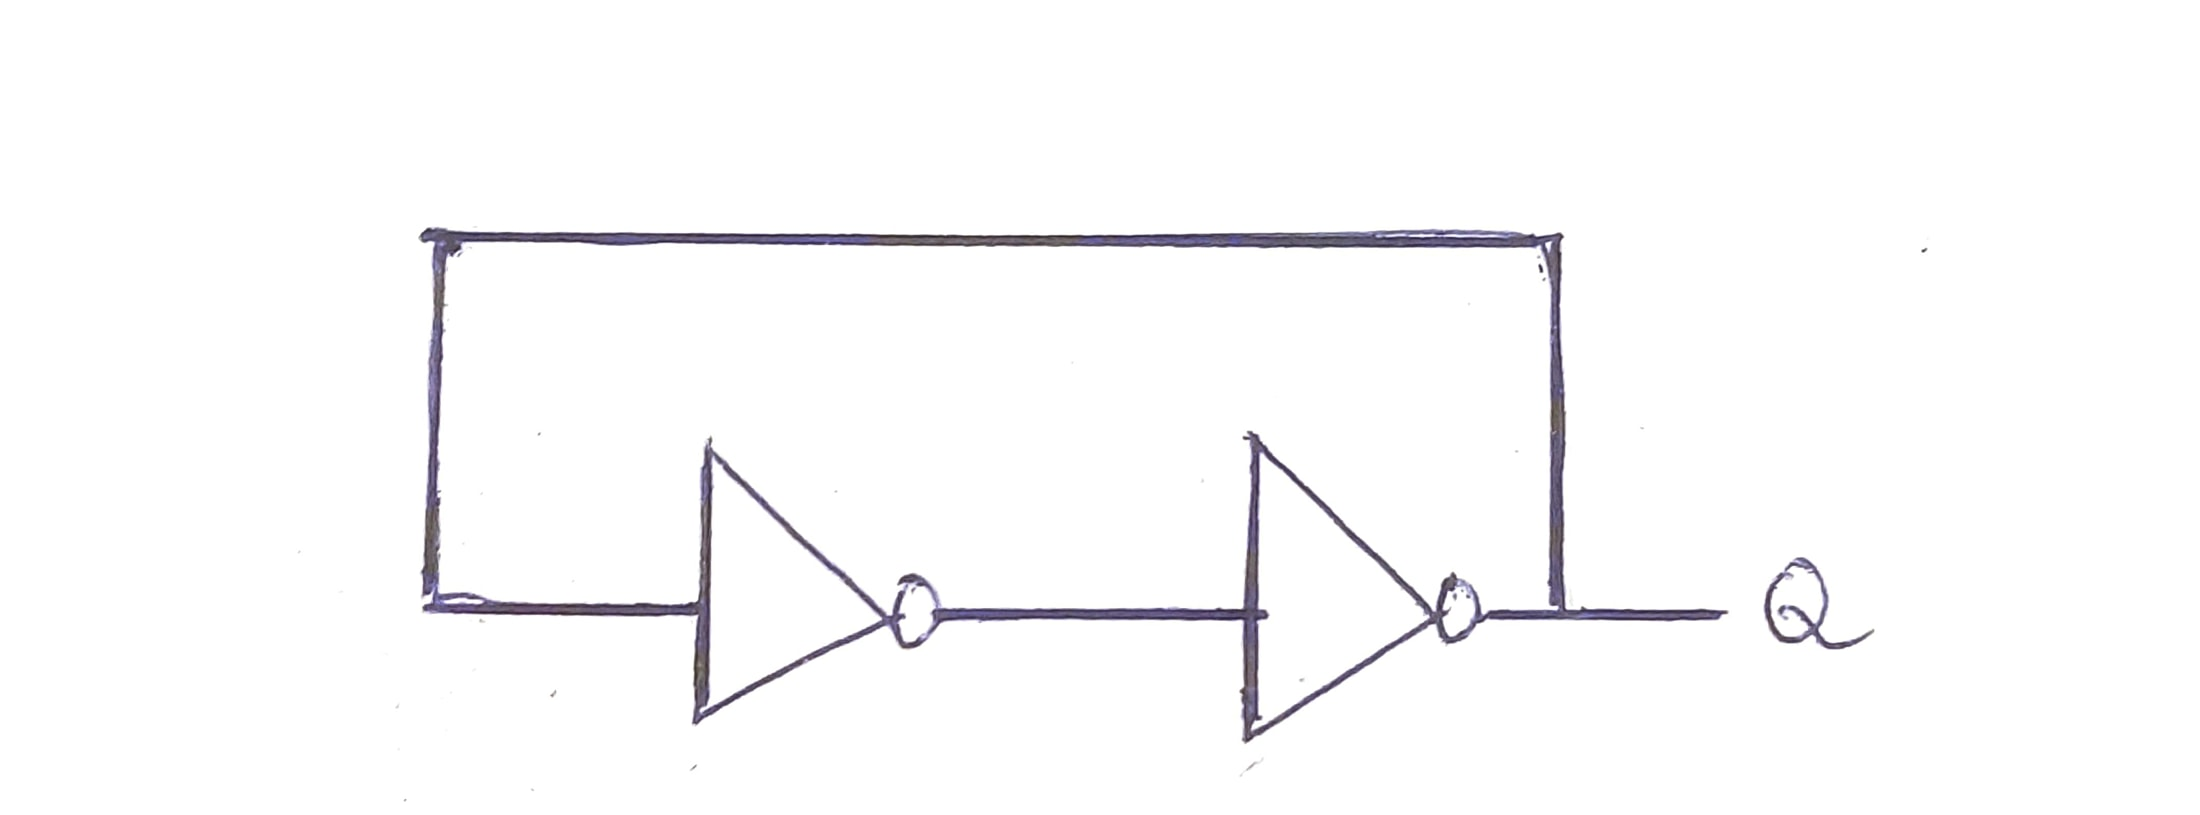
\includegraphics[scale = 0.16]{Documents/feedback_1.jpg}
\end{center}
\begin{center}
    \textbf{A Feedback Logic Circuit}
\end{center}
The memory elements that employ this sort of simple inverter feedback mechanism are called \textbf{\emph{Flip-Flops}}. A flip-flop circuit has two outputs, one for the normal value and one for the complement value of the stored bit. The inverting gates are the reason that the complementary outputs are always available. Binary information can enter a flip-flop in a variety of ways and gives rise to 
different types of flip-flops.
\par
\noindent
The \textbf{\emph{RS Flip Flop}} or the \textbf{\emph{Reset-Set Flip Flop}} is one of the simplest flip-flop memory elements. Following is an RS flip flop constructed using two NOR gates.
\begin{center}
    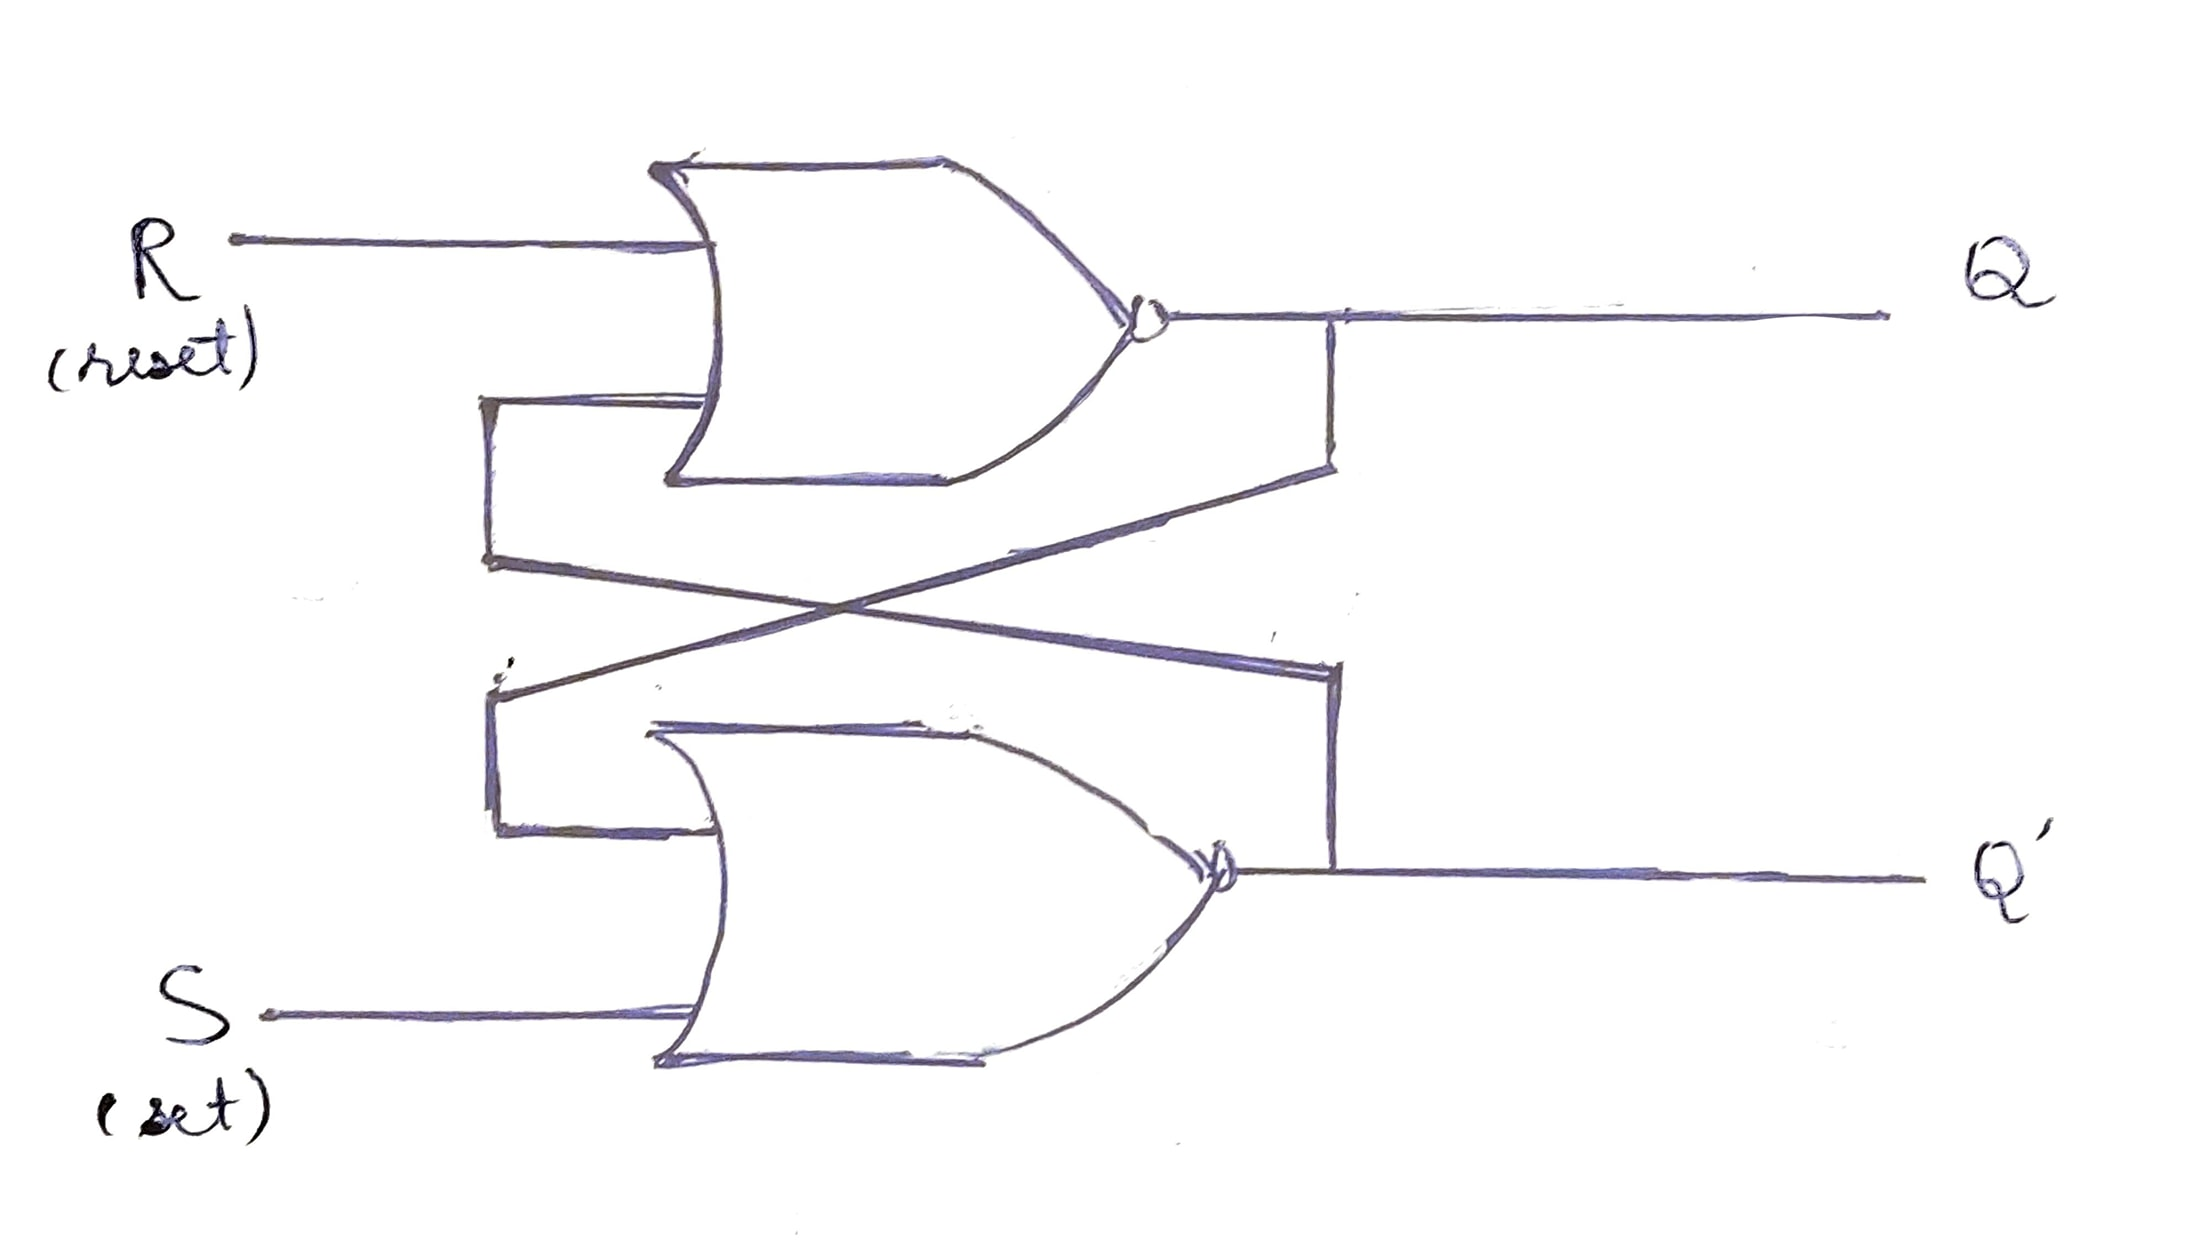
\includegraphics[scale = 0.14]{Documents/rsff_1.jpg}
\end{center}
\begin{center}
    \textbf{RS Flip Flop}
\end{center}
\noindent
It has two complementary outputs, $Q$ and $Q'$ and are referred to as the normal and complement outputs, 
respectively. When $Q = 1$ and $Q' = 0$, it is in the \emph{set state} (or 1-state). When $Q = 0$ and $Q' = 1$, it is in the \emph{reset/clear state} (or 0-state).
\newline
\noindent 
Sometimes, in usage of RS gates, it is desirable that state change only happens when certain conditions are met regardless of the condition of either the \emph{set} or the \emph{reset} inputs. Thus, a \textbf{\emph{gates RS Flip Flop}} can be constructed by adding an extra conditional input called the \emph{enabler} (EN). It can be connected to a \emph{clock} to be operated as a \emph{latch}. The outputs are only activated when a logic "1" is applied to its EN input and deactivated by a 
logic "0". Following is the circuit diagram for the gated RS flip-flop.
\begin{center}
    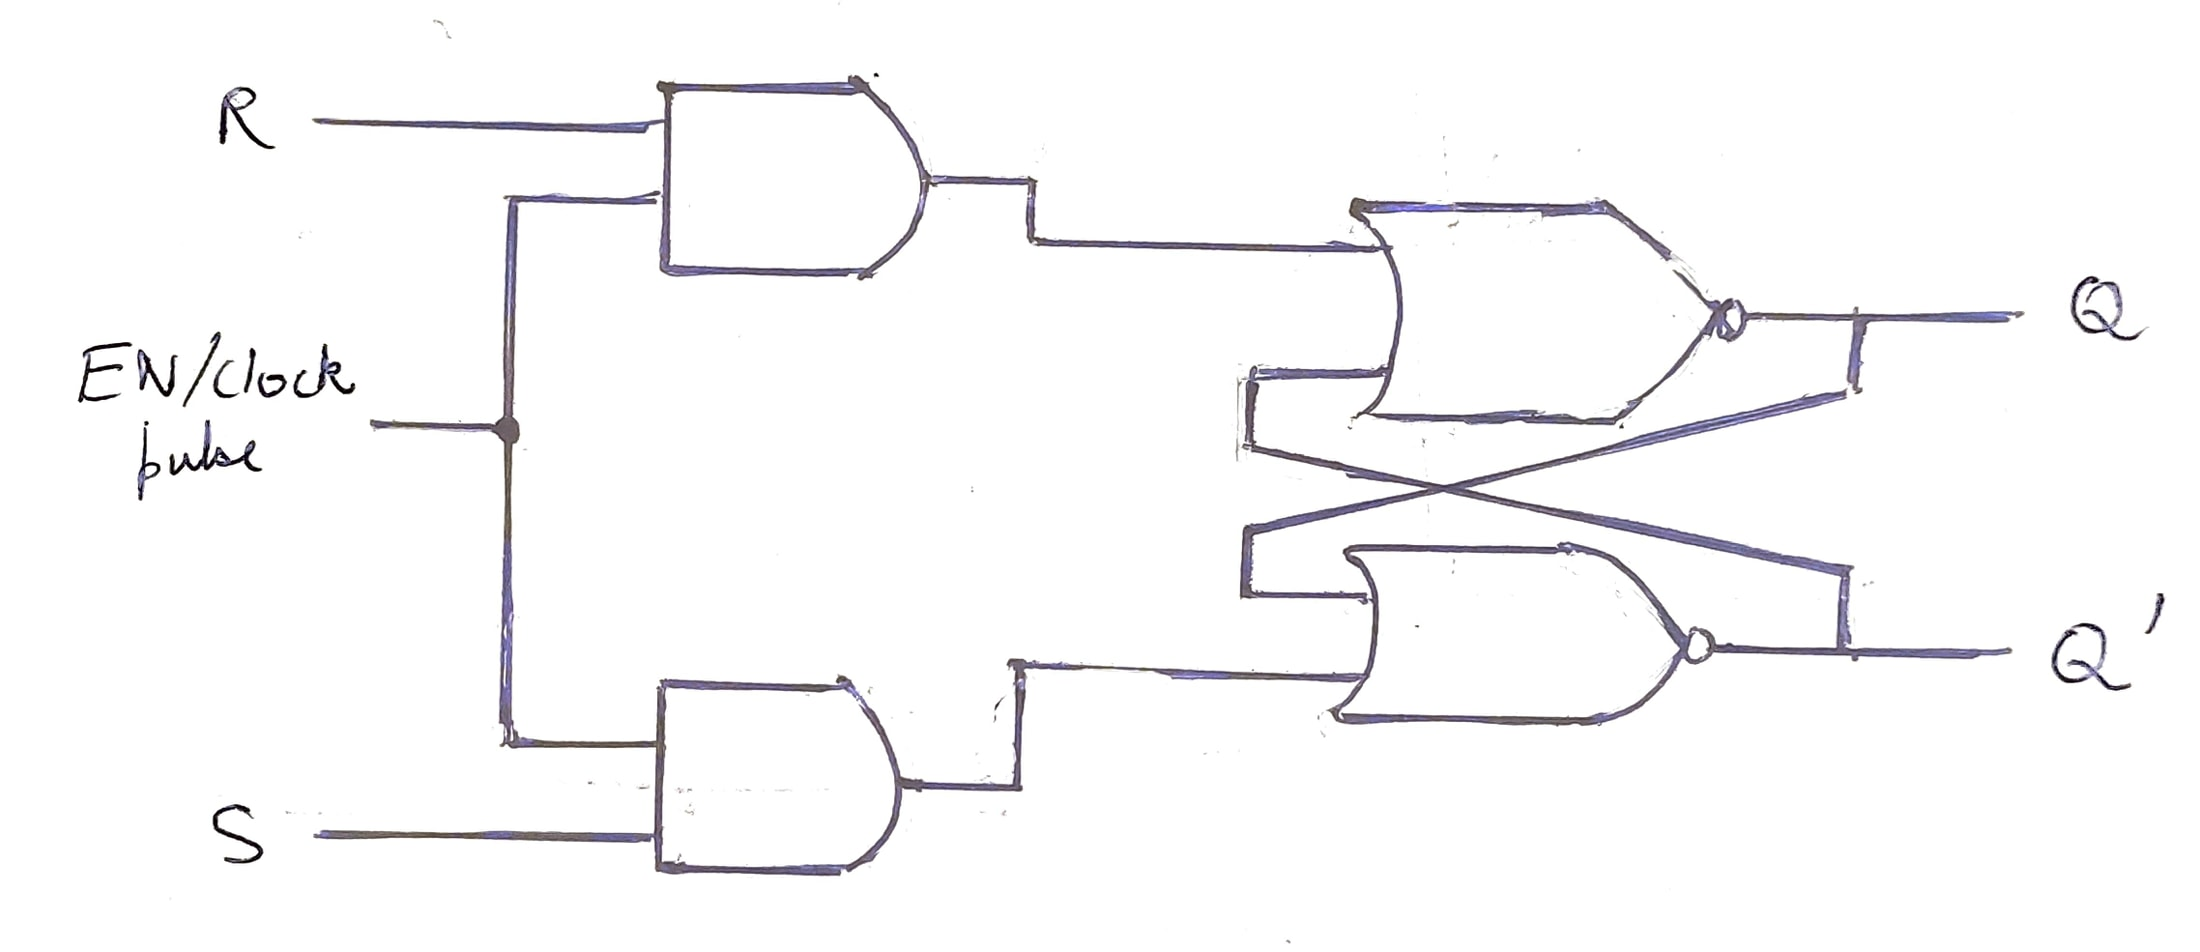
\includegraphics[scale = 0.16]{Documents/clockedrsff_1.jpg}
\end{center}
\begin{center}
    \textbf{Gated or Clocked RS Flip Flop}
\end{center}
The RS flip-flop can be modified to eliminate some of its shortcomings by converting it into a \textbf{\emph{D Flip Flop}} or \textbf{\emph{Data Flip Flop}}. The D flip-flop has only a single data input $D$, which is connected to the $S$ input of an RS 
flip-flop, while the inverse of $D$ is connected to the $R$ input. Again, the D flip-flop has an \emph{enabler} input which plays a similar function as it plays in the gated RS flip-flop.
\begin{center}
    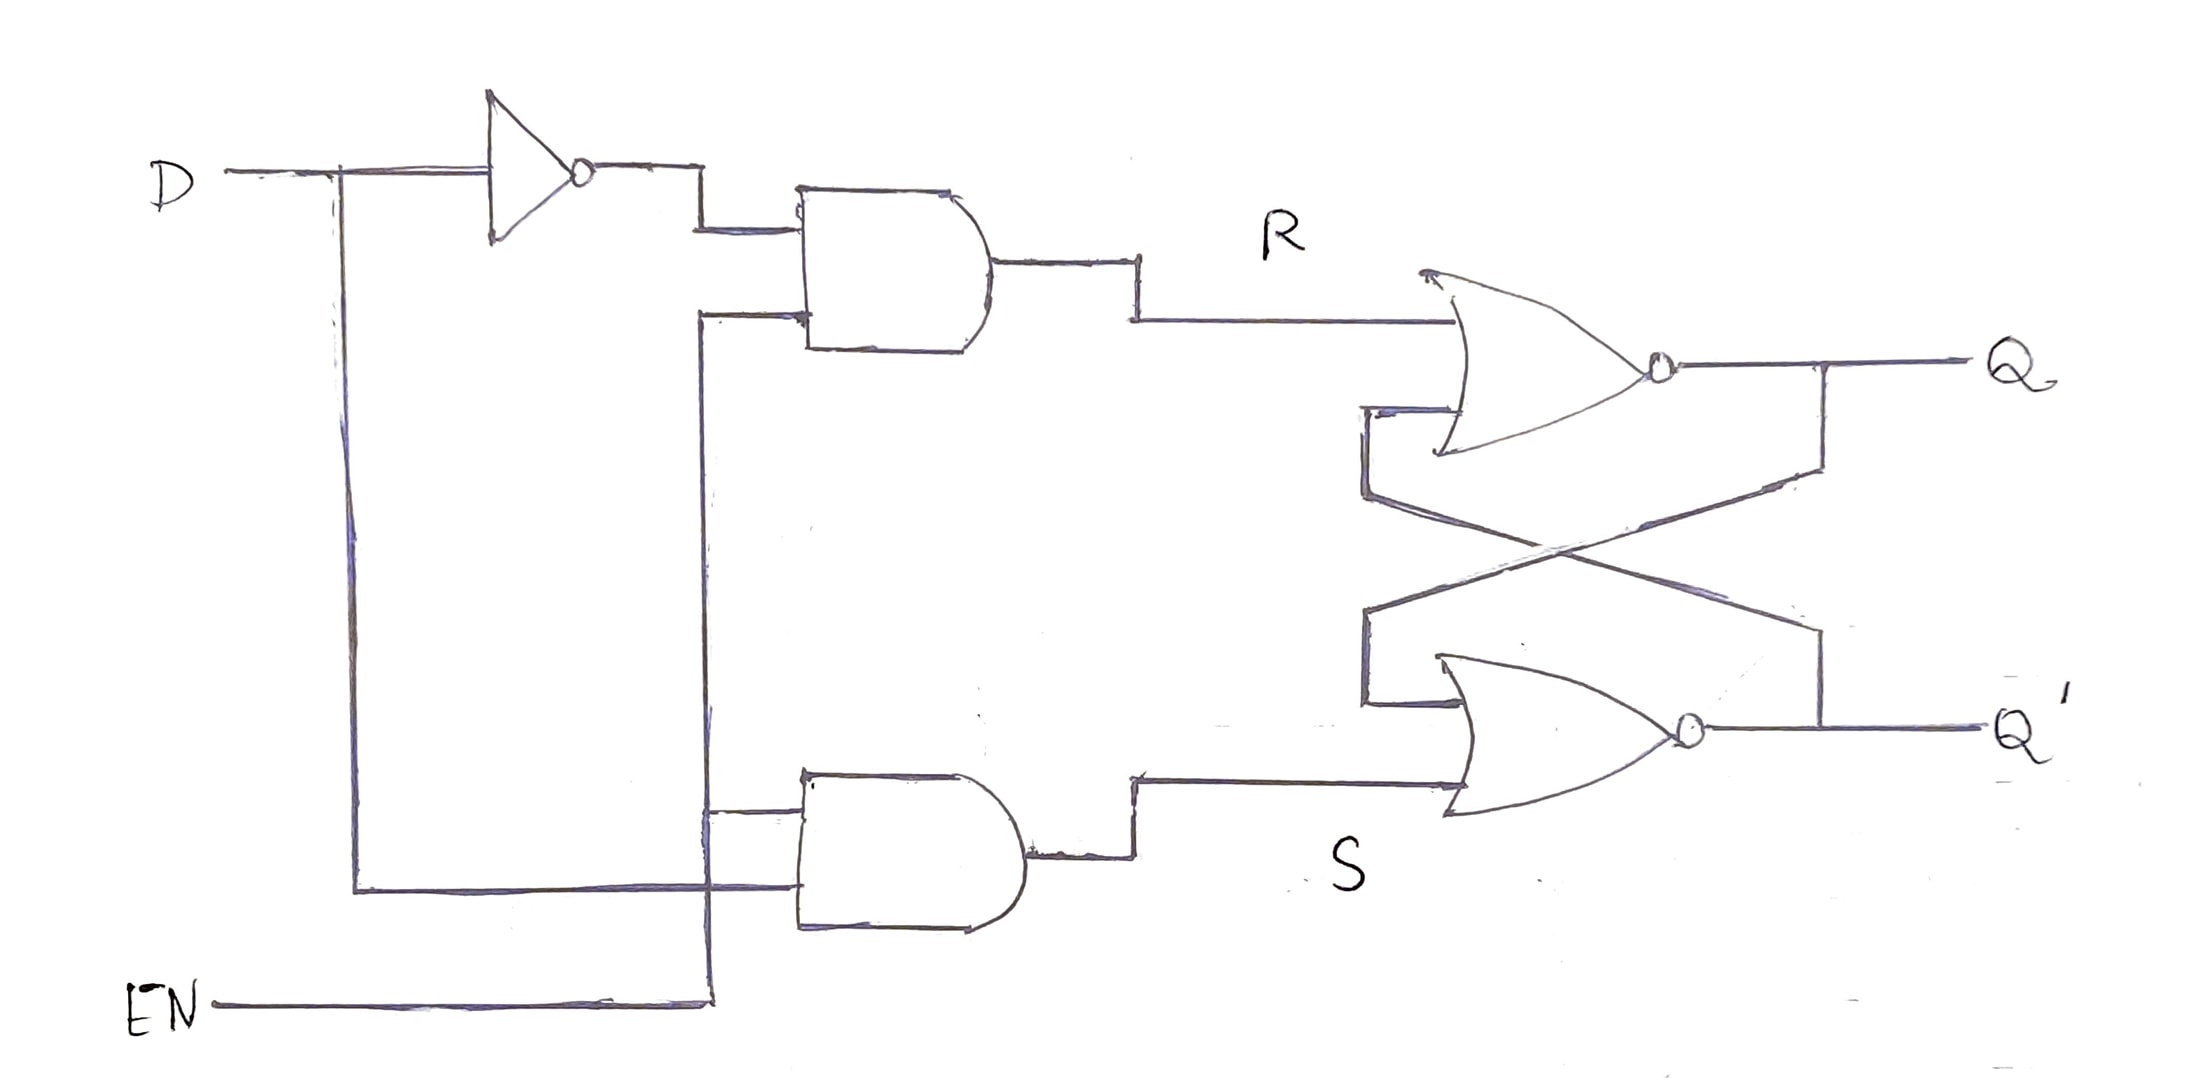
\includegraphics[scale = 0.18]{Documents/dff_1.jpg}
\end{center}
\begin{center}
    \textbf{D Flip Flop}
\end{center}
The \textbf{\emph{JK Flip Flop}} (JK stands for Jack Kilby, its inventor) is one of the most widely used flip-flops. Similar to the RS flip-flop, it has two data inputs ($J$ and $K$) and an \emph{enabler} pulse input. The JK flip-flop eliminates all the indeterminate case possibilities that the RS flip-flop has, thus having a clear advanatge over it.
\begin{center}
    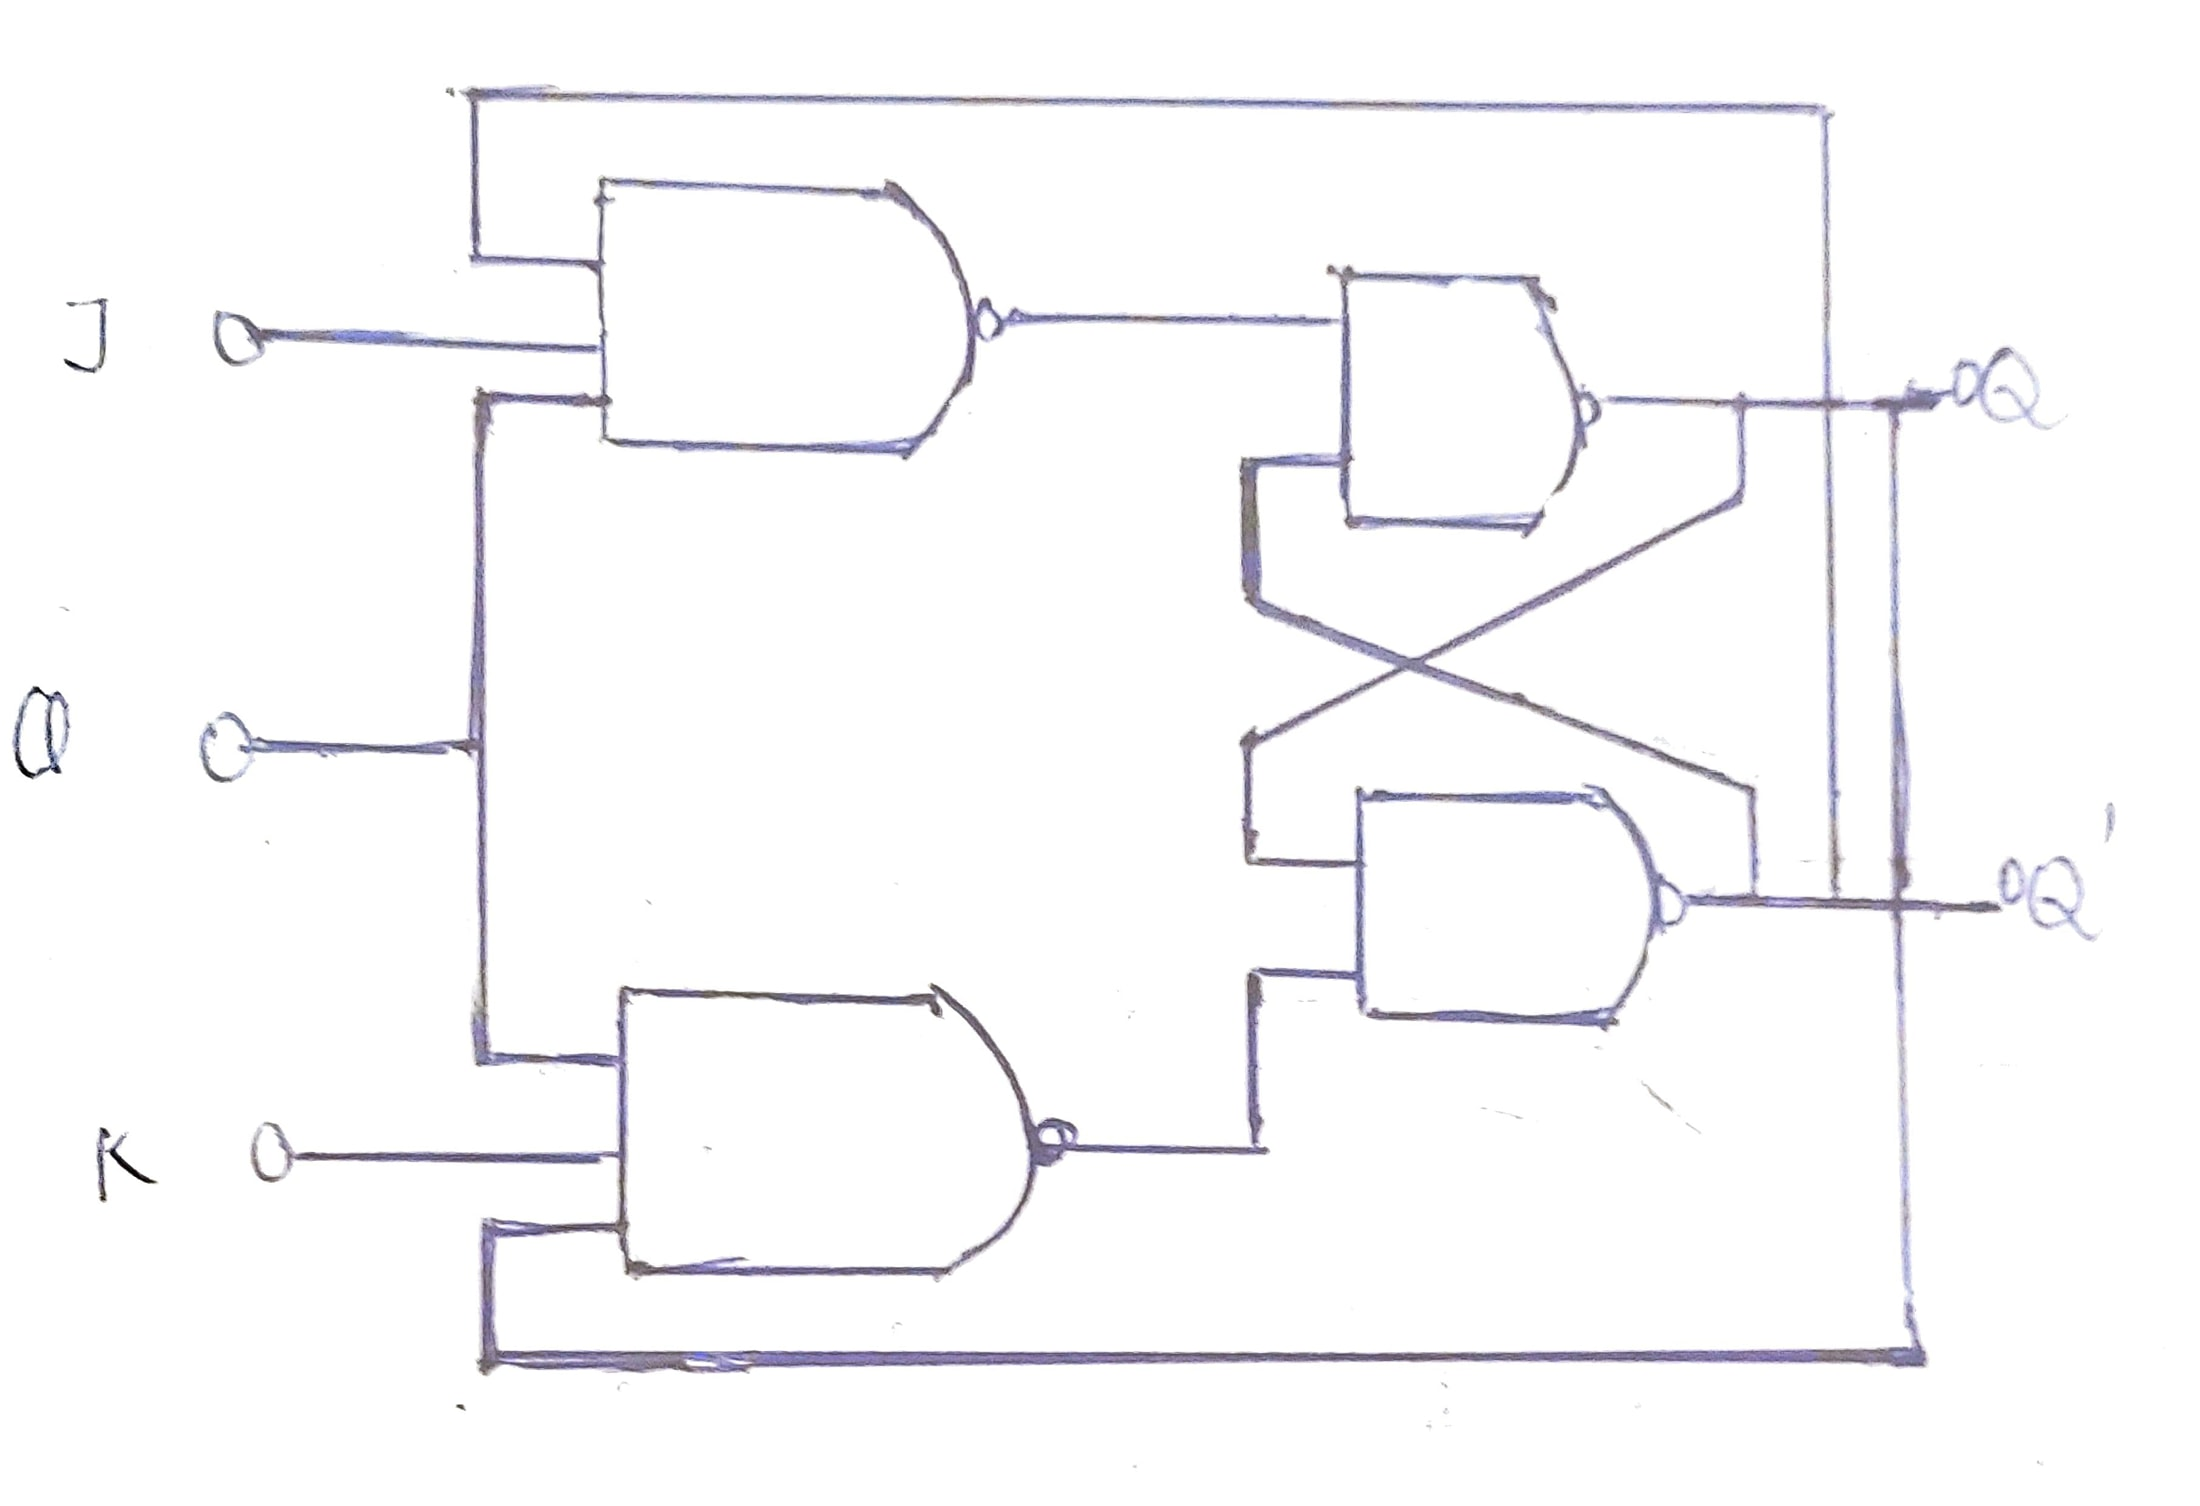
\includegraphics[scale = 0.16]{Documents/jkff_1.jpg}
\end{center}
\begin{center}
    \textbf{JK Flip Flop}
\end{center}
The JK flip-flop can be extended by adding another cascade of a \emph{latch} RS circuit. So, two RS flip-flops connected in in series, one for the \emph{Master} circuit, which triggers on the leading edge of the clock pulse and the other, the \emph{Slave} circuit, which triggers on the falling edge of the clock pulse. The main advantage of the \textbf{\emph{Master Slave JK Flip Flop}} is that it eradicates the timing problems of the circuit. The timing problems are referred to as \emph{race conditions}.
\begin{center}
    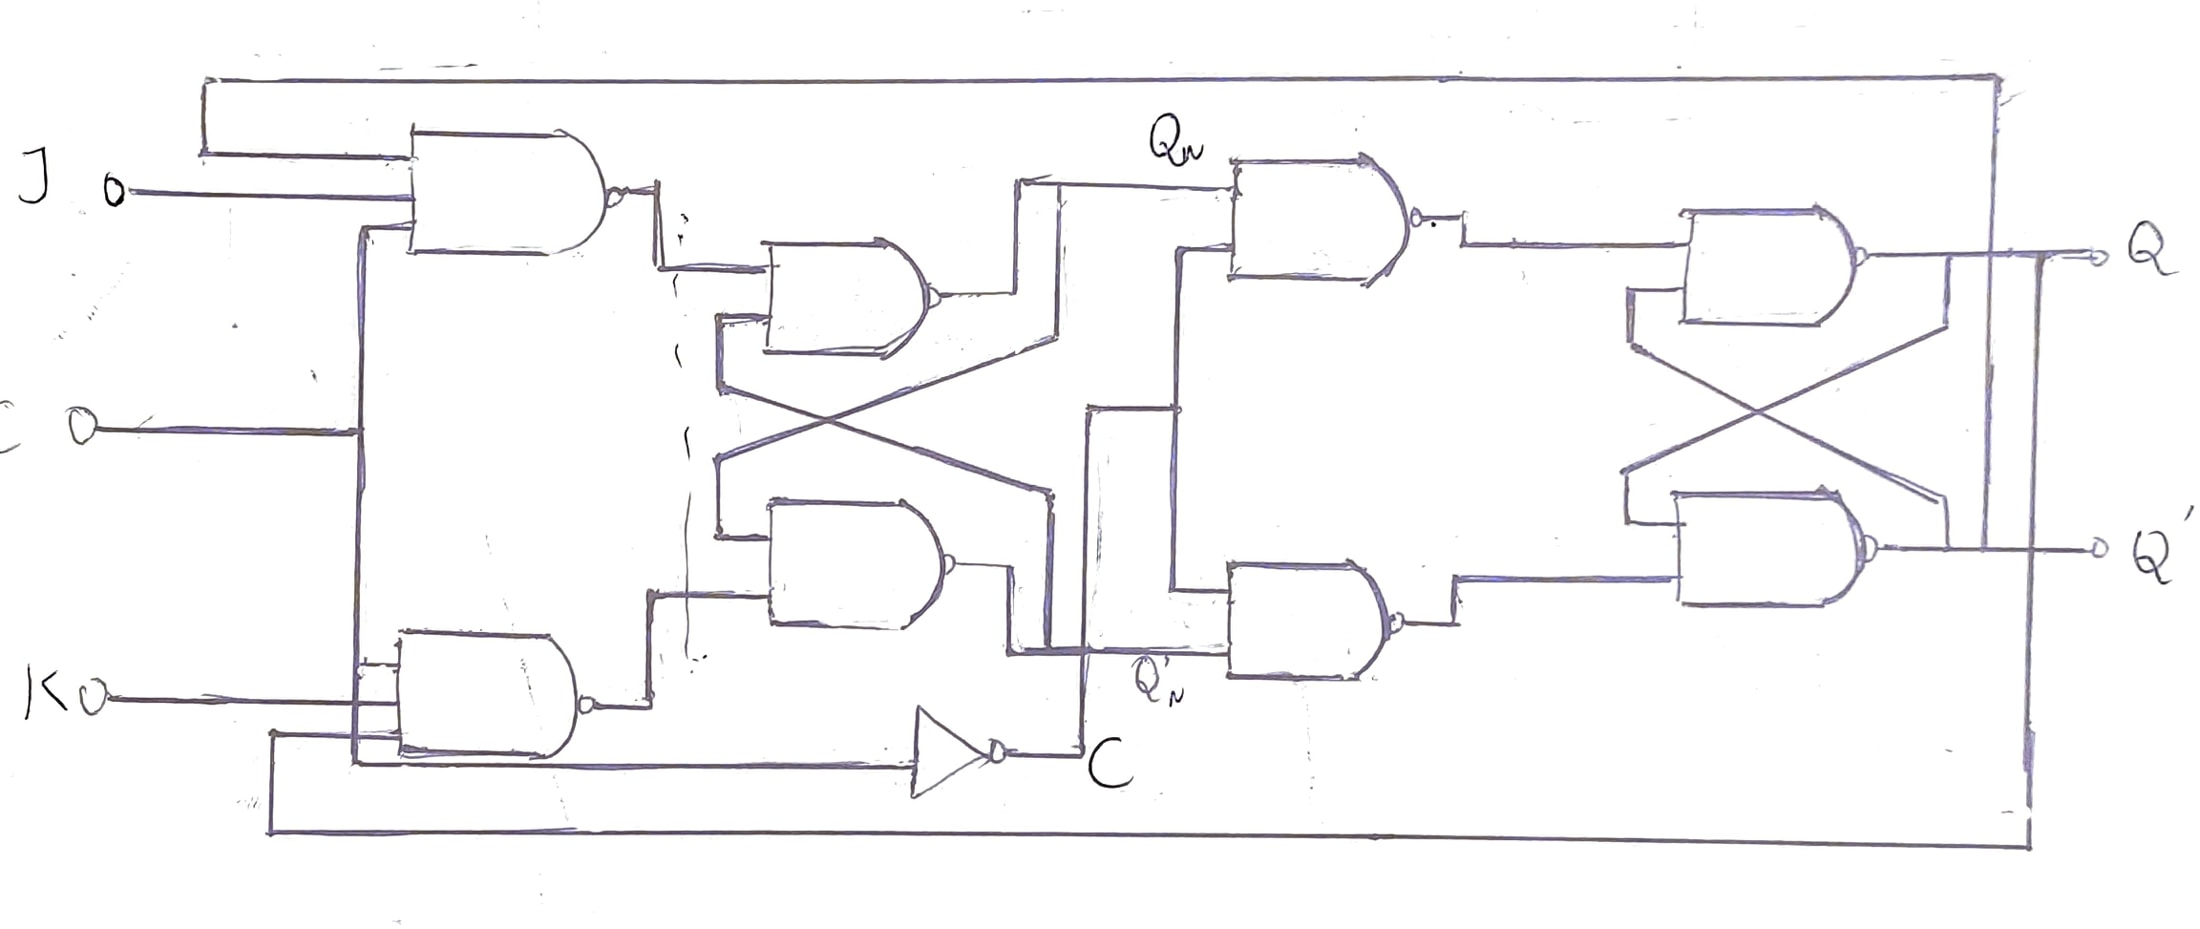
\includegraphics[scale = 0.2]{Documents/msjkff_1.jpg}
\end{center}
\begin{center}
    \textbf{Master Slave JK Flip Flop}
\end{center}
If both of the two inputs of the Master Slave JK flip-flop are $1$ then we call it \textbf{\emph{T Flip Flop}}.
\section{Observations}
\begin{center}
    \textbf{Characteristic Table for RS Flip Flop}
\end{center}
\begin{center}
    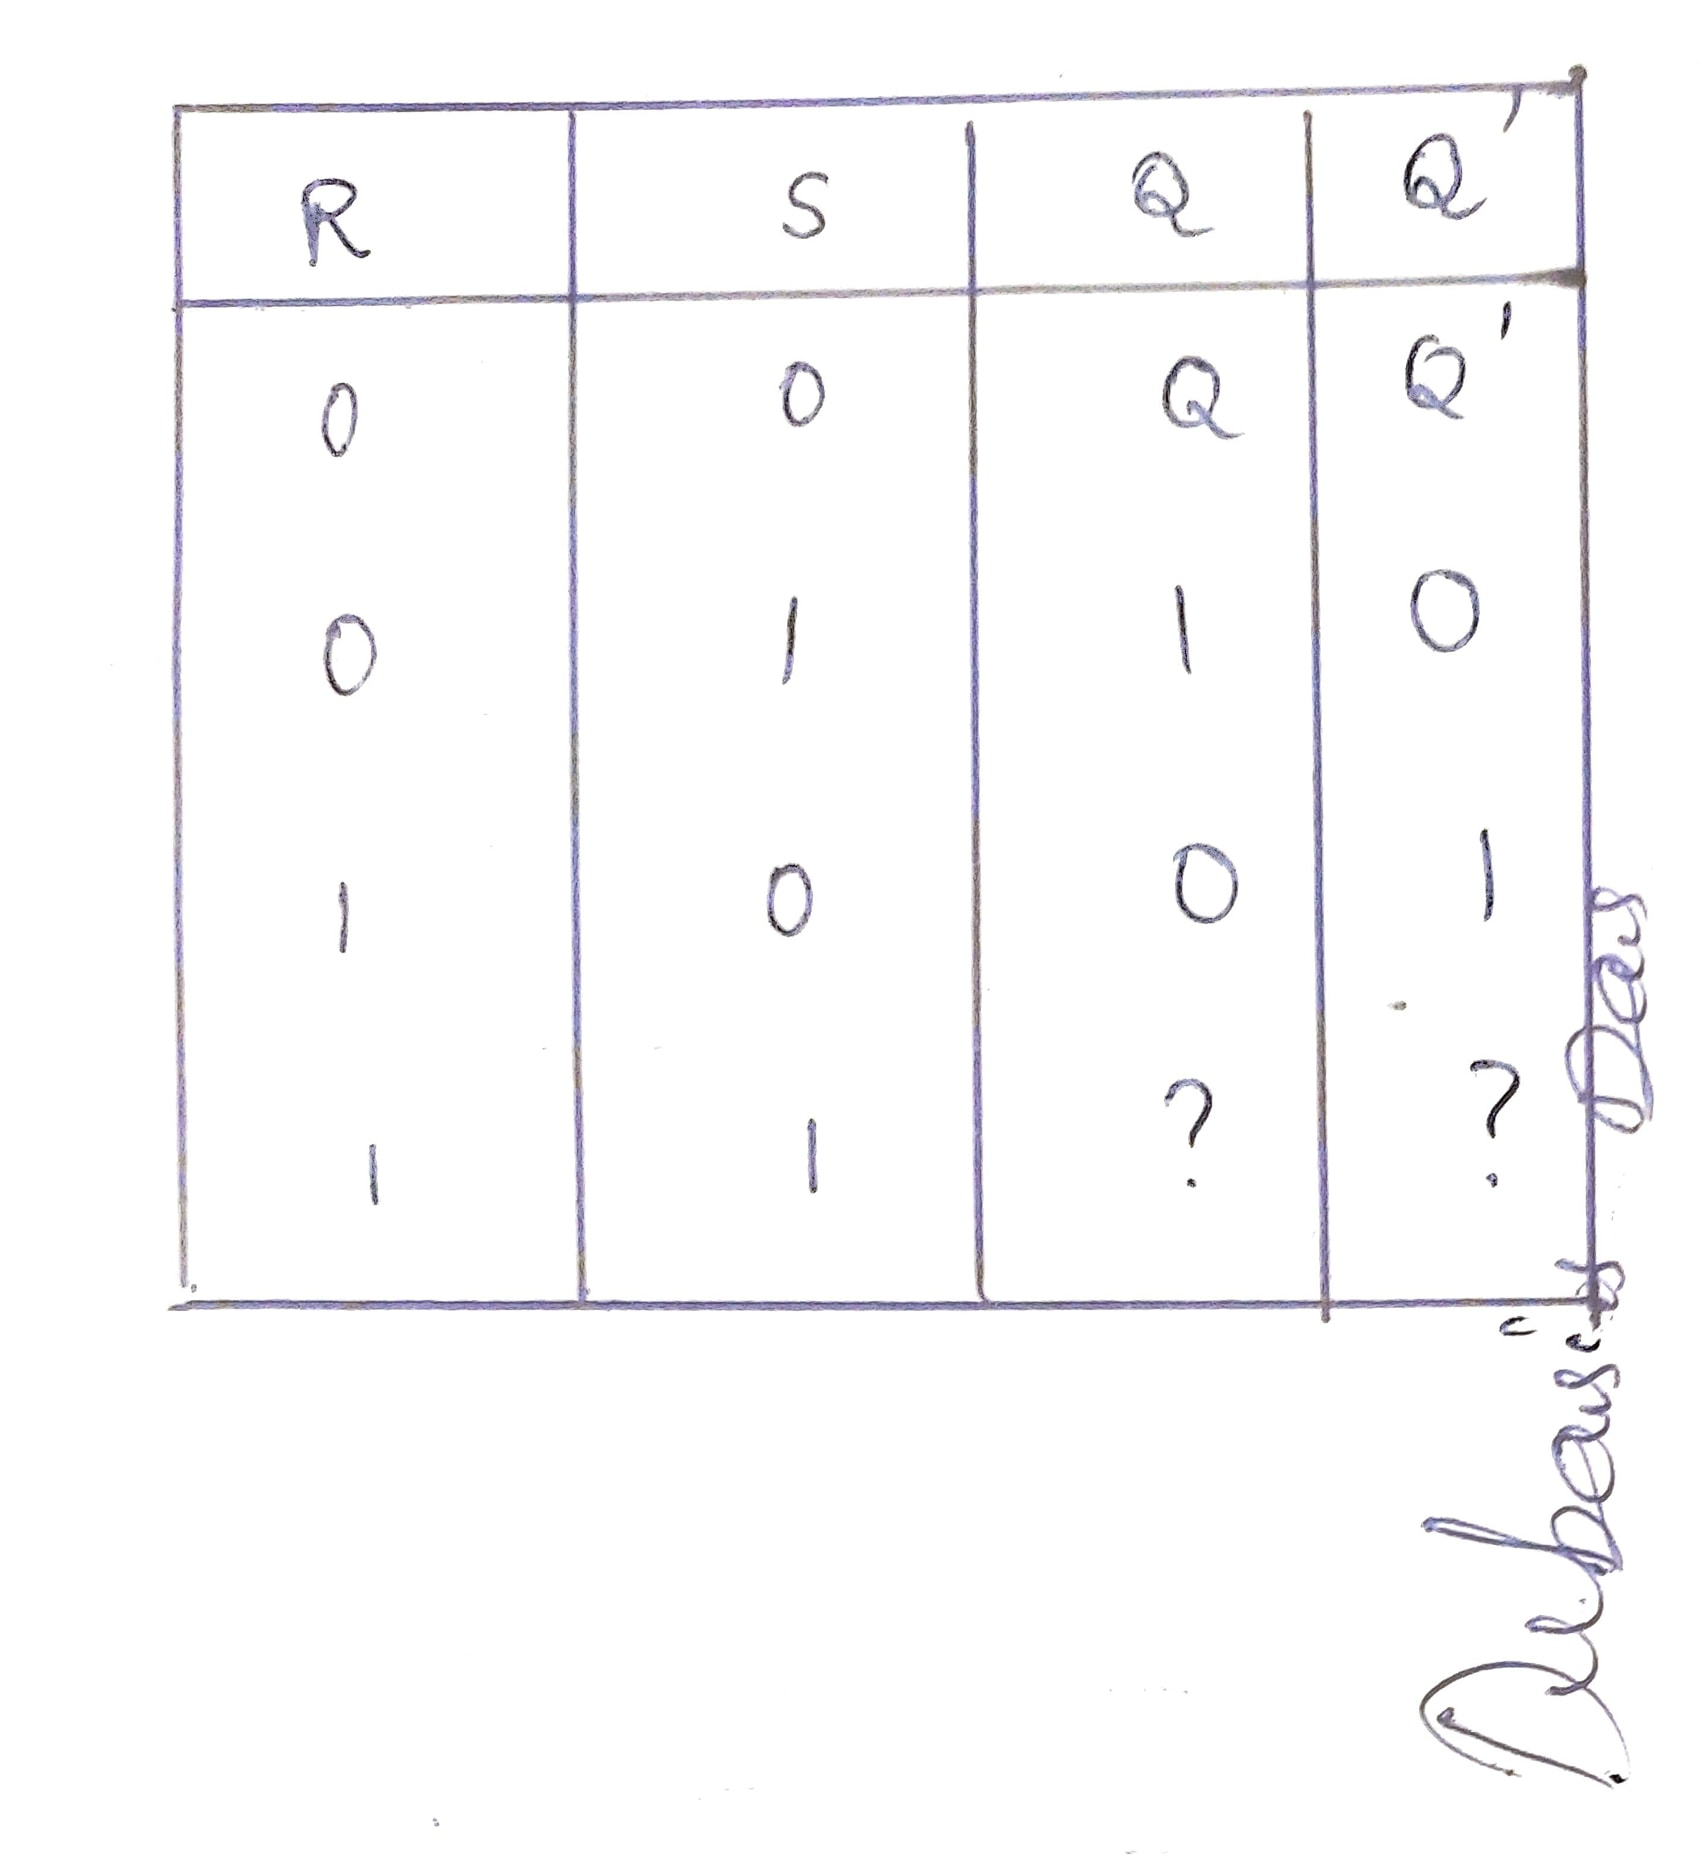
\includegraphics[scale = 0.15]{Documents/tabrs_1 (1).jpg}
\end{center}
\clearpage
\begin{center}
    \textbf{Characteristic Table for Gated or Clocked RS Flip Flop}
\end{center}
\begin{center}
    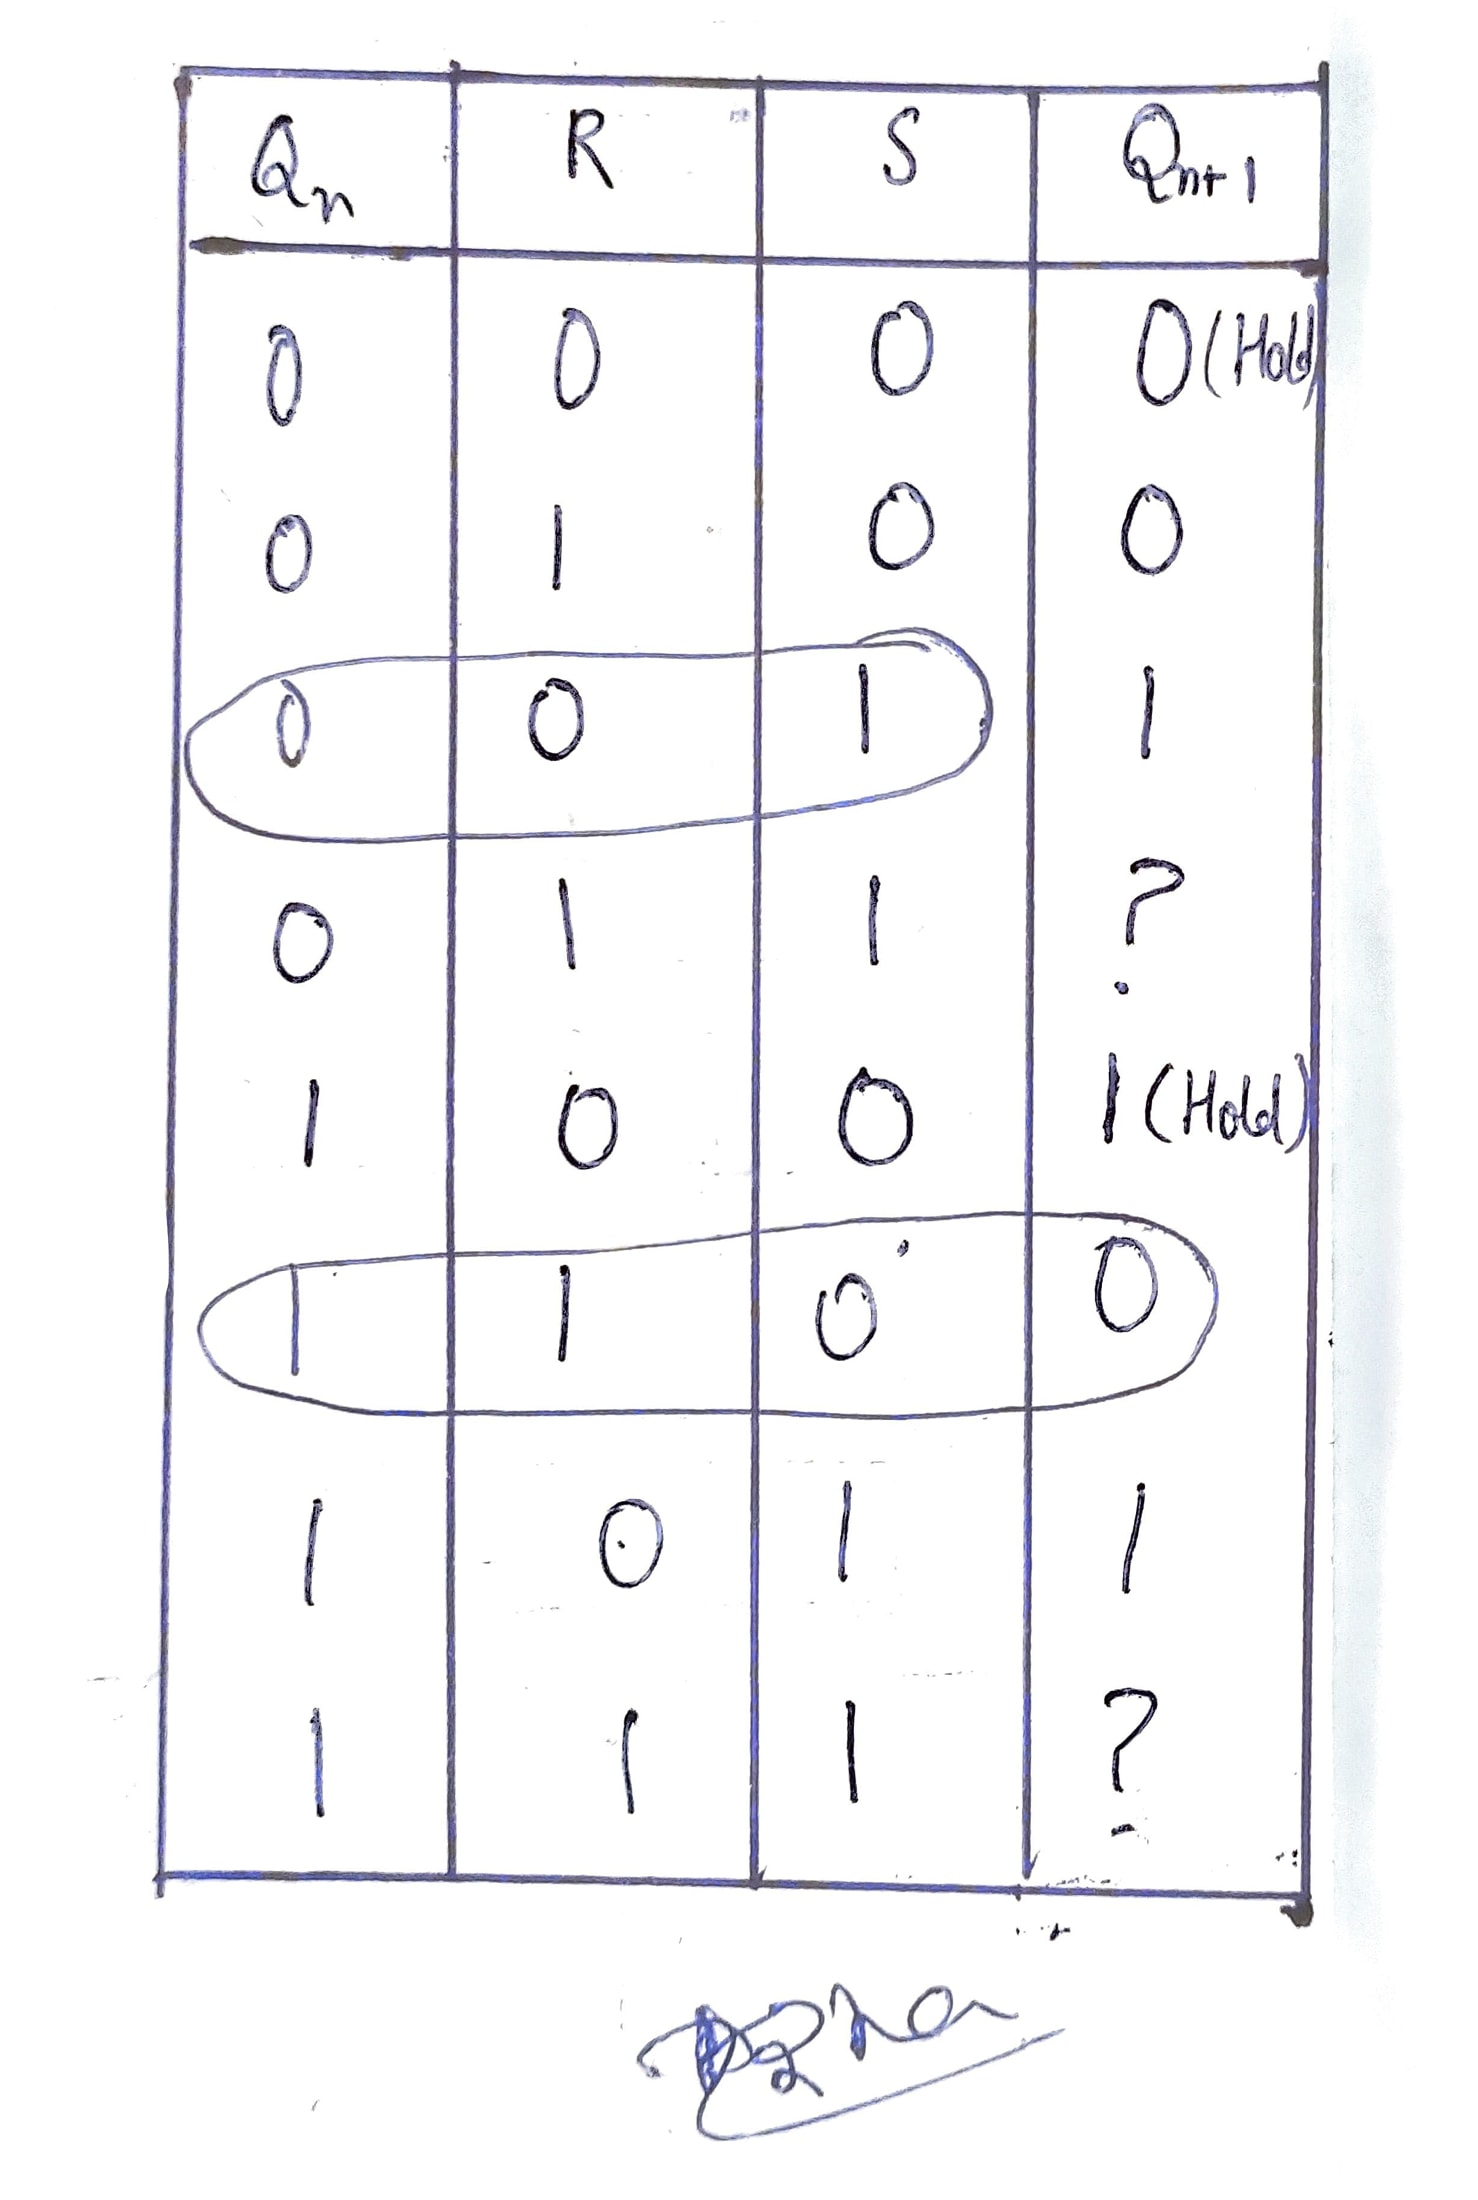
\includegraphics[scale = 0.15]{Documents/tabrsclocked_1.jpg}
\end{center}
\begin{center}
    \textbf{Characteristic Table for D Flip Flop}
\end{center}
\begin{center}
    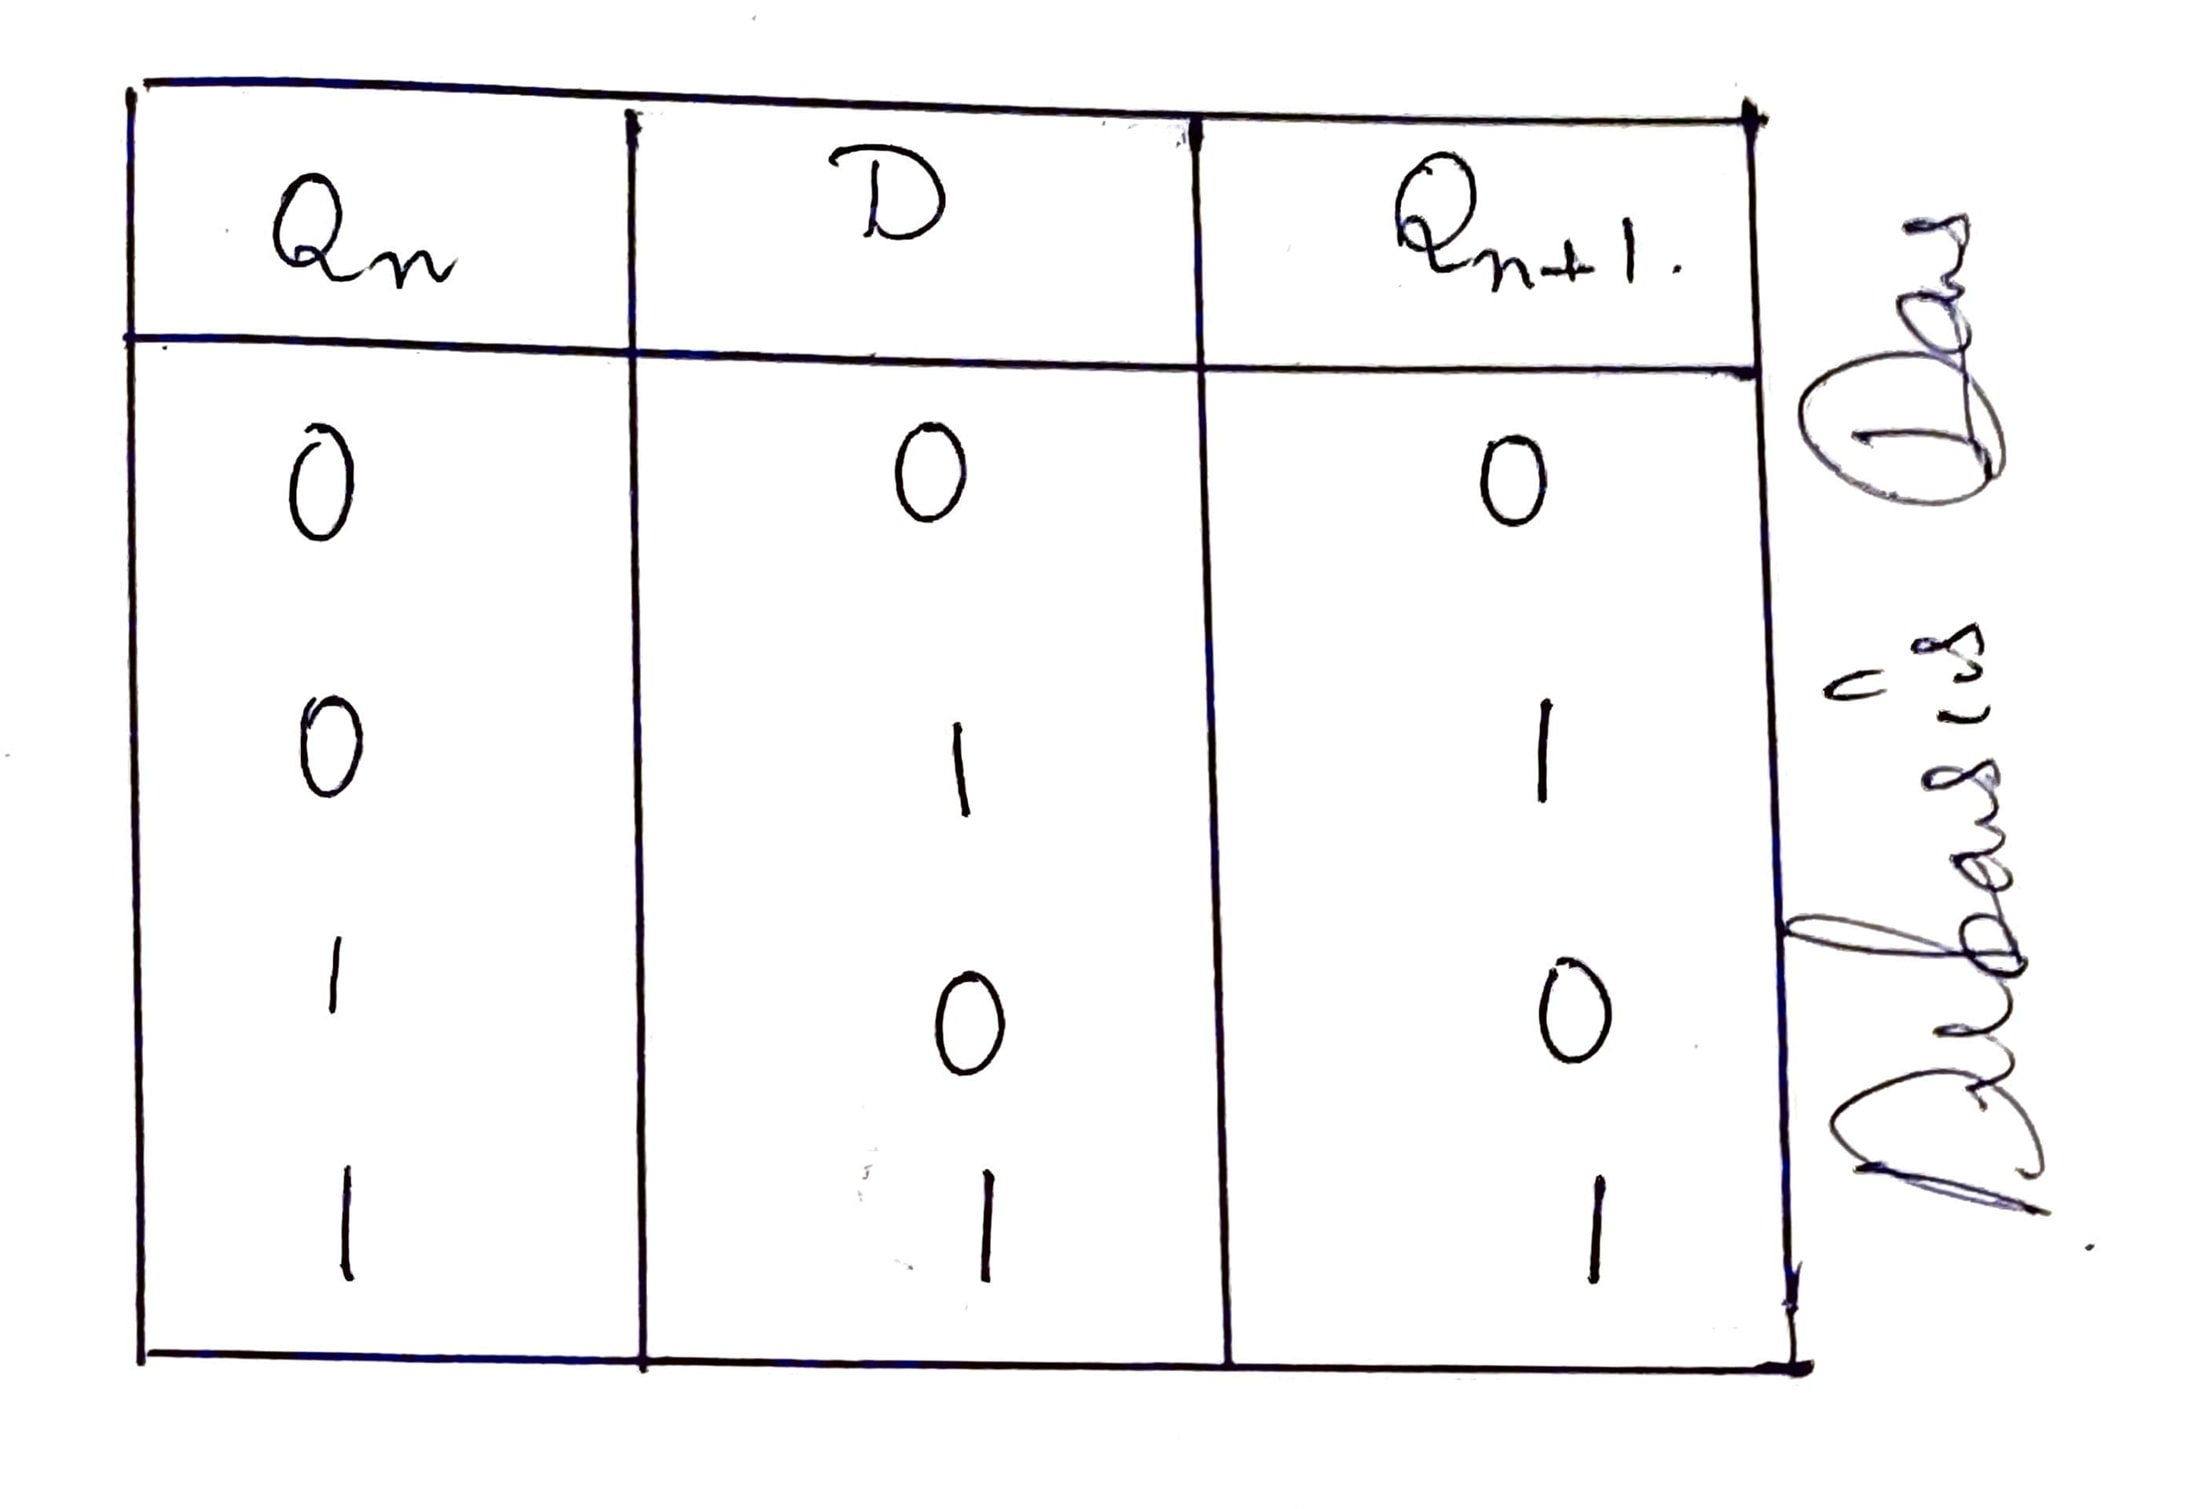
\includegraphics[scale = 0.1]{Documents/tabd_1.jpg}
\end{center}
\clearpage
\begin{center}
    \textbf{Characteristic Table for JK Flip Flop}
\end{center}
\begin{center}
    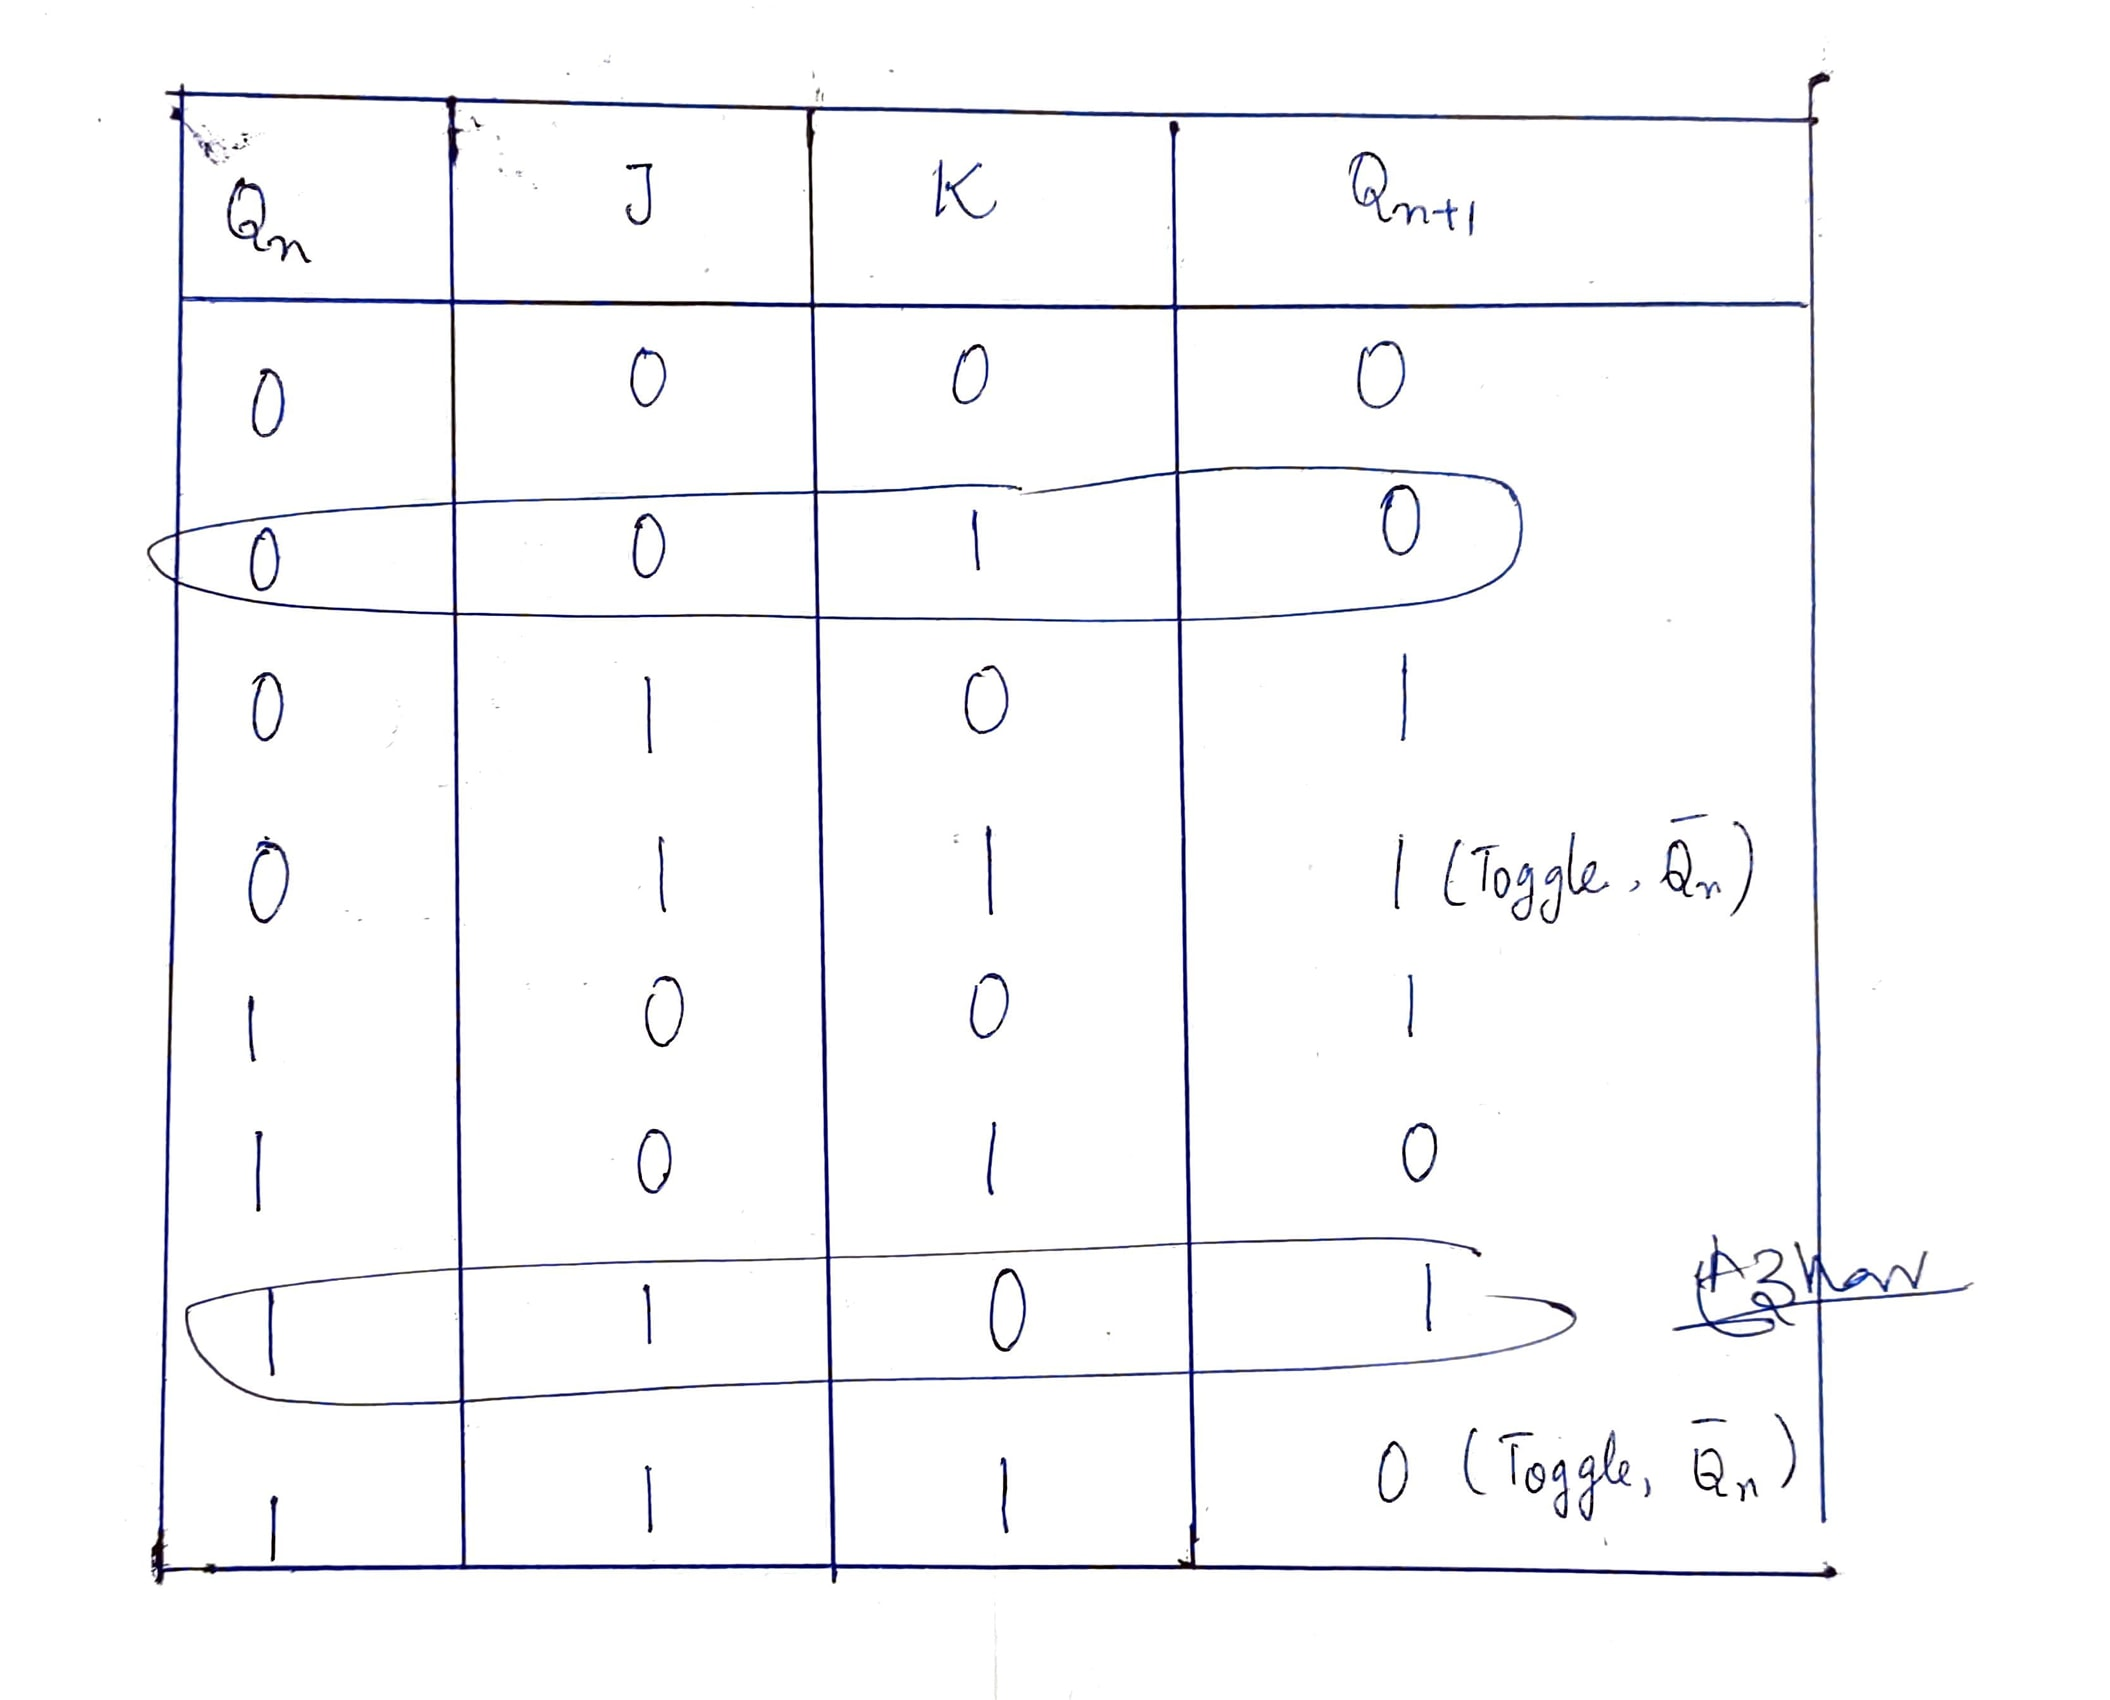
\includegraphics[scale = 0.15]{Documents/tabjk_1.jpg}
\end{center}
\begin{center}
    \textbf{Characteristic Table for Master Slave JK Flip Flop}
\end{center}
\begin{center}
    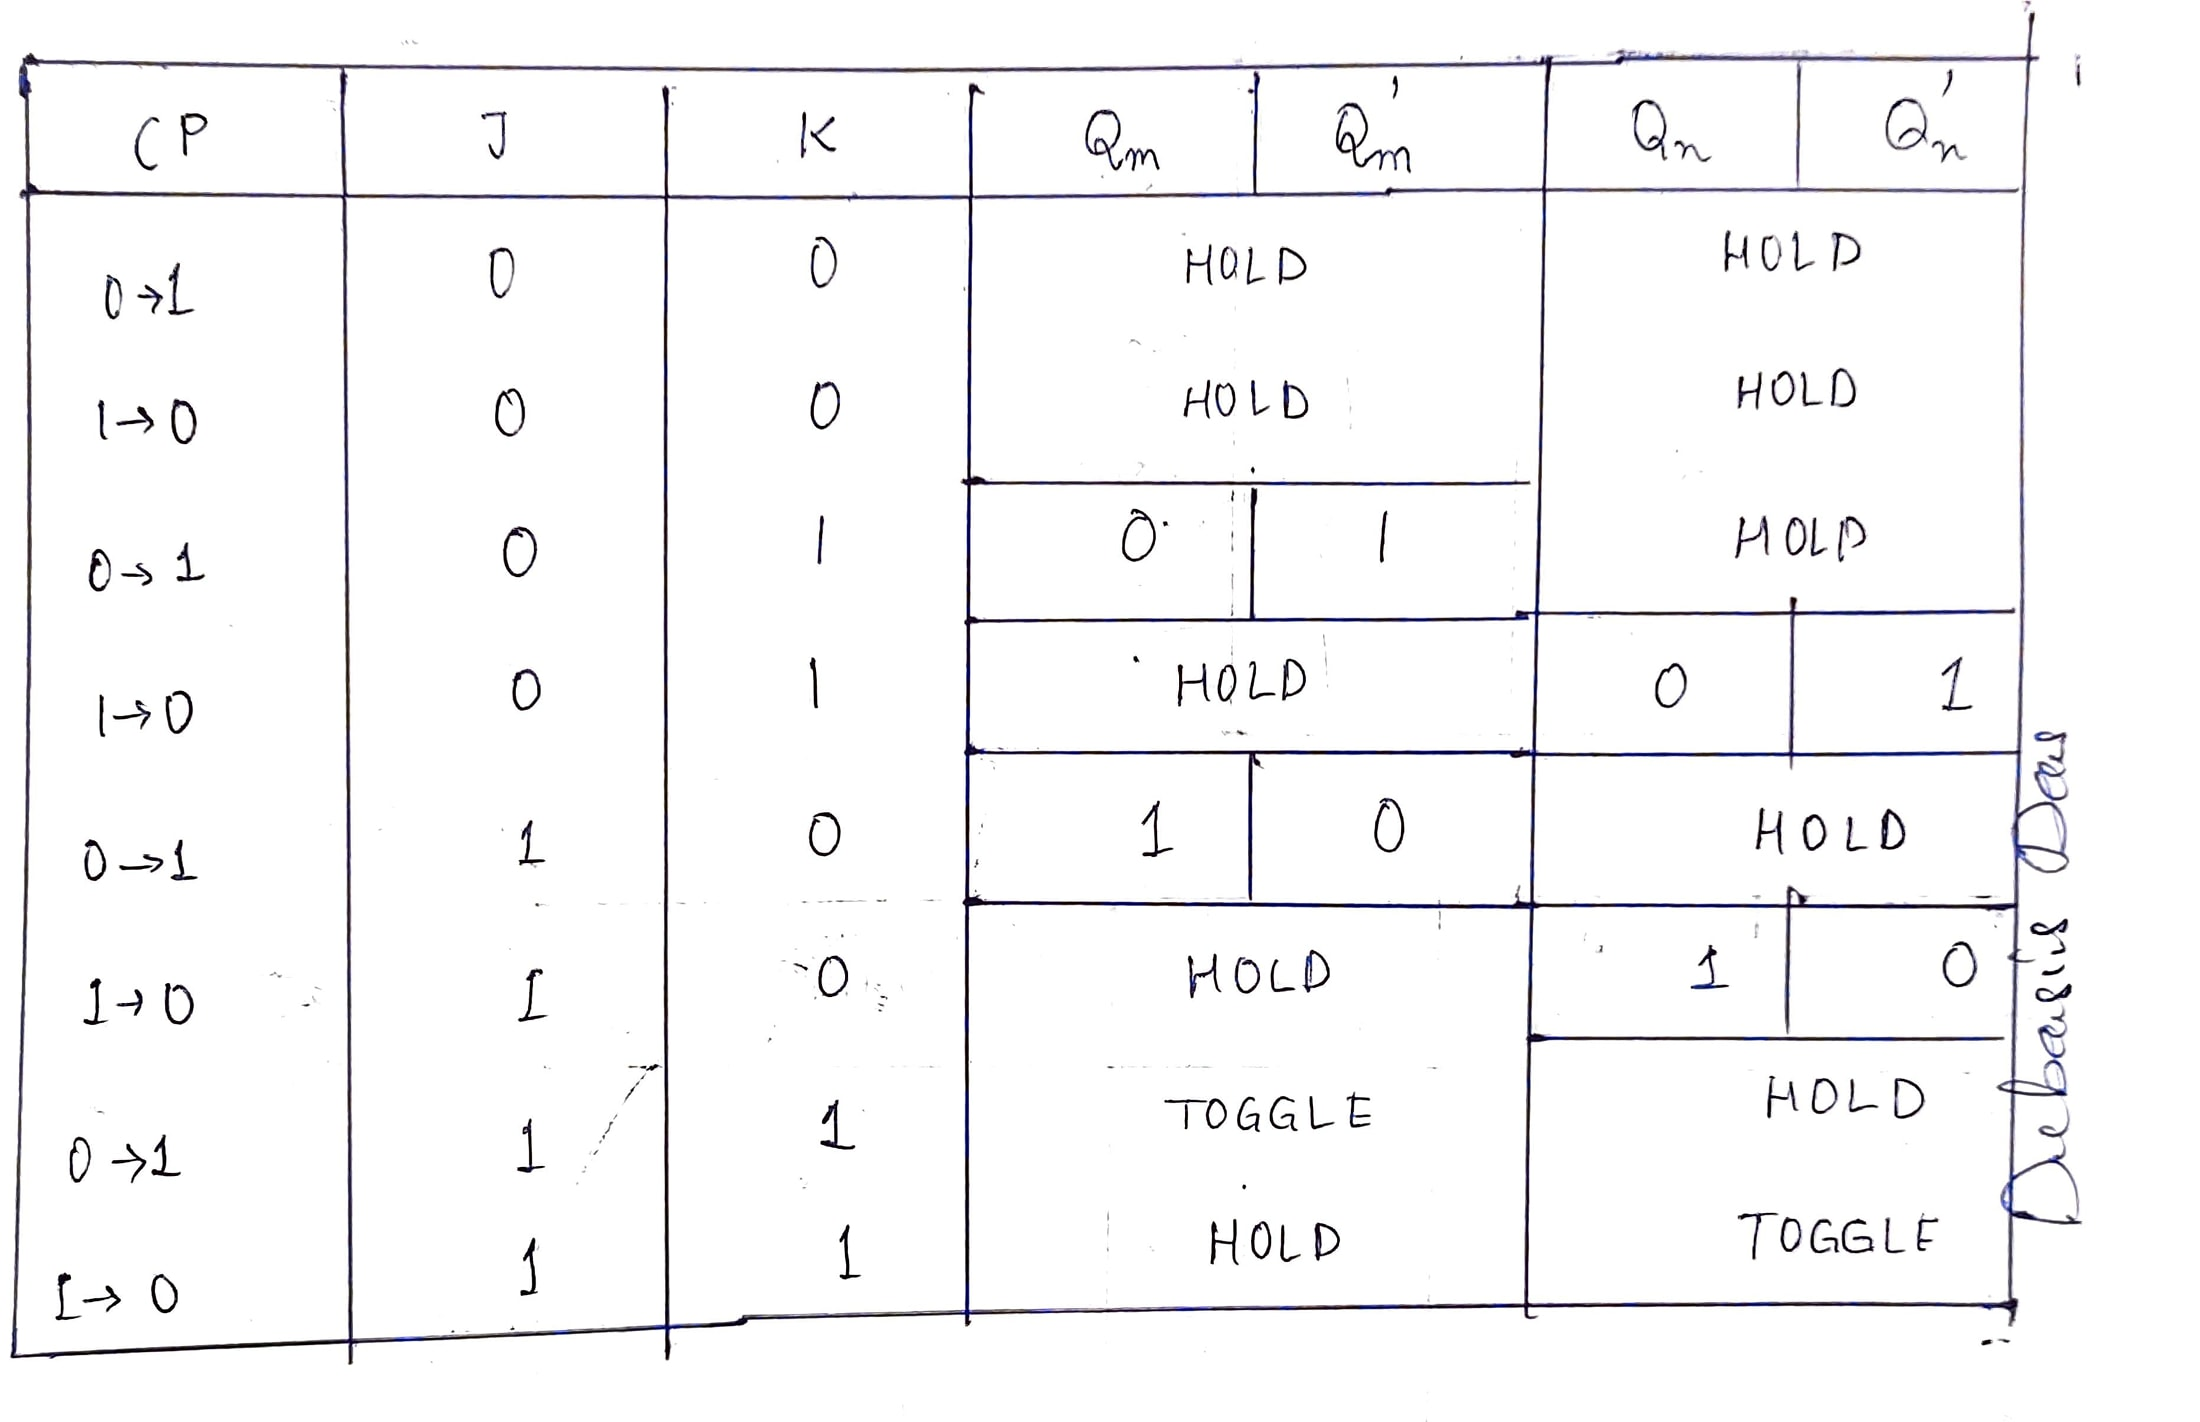
\includegraphics[scale = 0.19]{Documents/tabms_1.jpg}
\end{center}
\clearpage
\begin{center}
    \textbf{Characteristic Table for T Flip Flop}
\end{center}
\begin{center}
    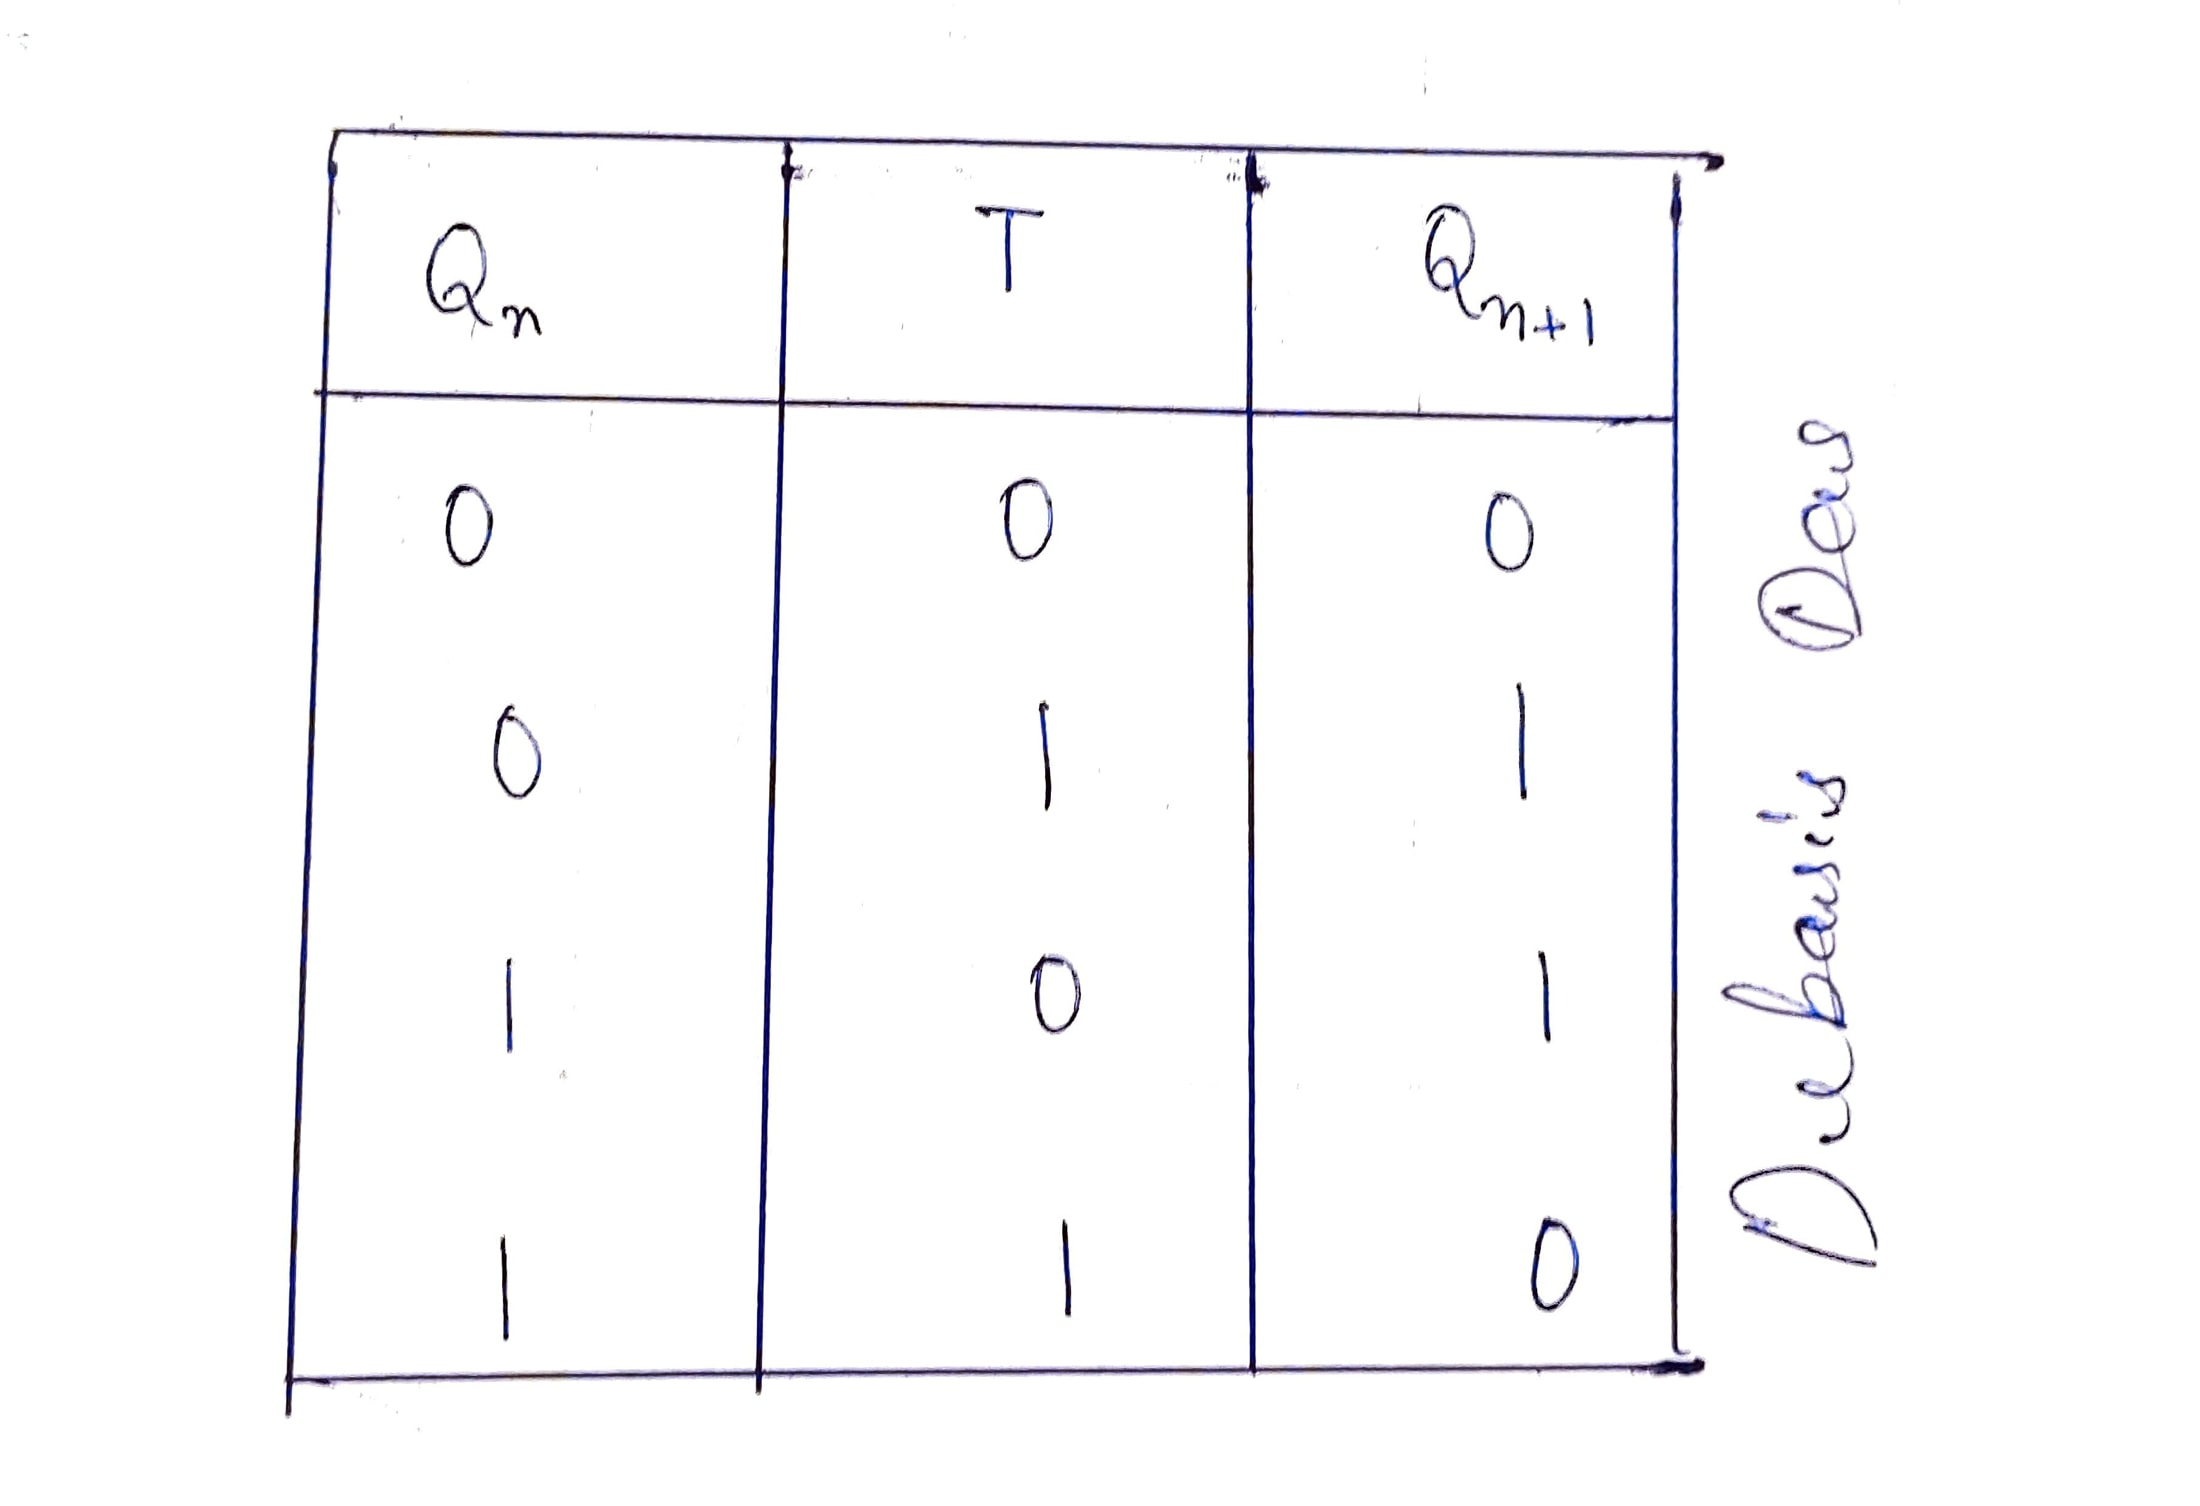
\includegraphics[scale = 0.15]{Documents/1616517802679.jpg}
\end{center}
\section{Result}
\begin{enumerate}
    \item The logic gate truth tables are obtained as enumerated under Observations section
\end{enumerate}
\section{Discussions}
\begin{enumerate}
    \item The working of RS flip flop can now be understood clearly. When $S = 1$ and $R = 0$ or when $S = 0$ and $R = 1$, the outputs can easily be understood by using Boolean algebra.
    \item But when $S = 0$ and $R = 0$, the RS flip-flop will \emph{hold} its previous state (whatever that might be.)
    \item We observe that $S = 1$ and $R = 1$ is an uunsatble configuration, thus making this set of inputs a disadvantage of the RS flip- flop.
    \item The main inference from the working of the Gated or Clocked RS flip-flop can be summarised as a RS flip-flop with a \emph{clock signal} attached to it.
    \item In case of the D flip-flop, when the $EN = 0$, the state is always held. When $EN = 1$, the output $Q$ follows the input $D$. And when $EN$ is turned back to zero state, the most recent $D$ input is remembered.
    \item In case of JK flip-flop, if one of the input is logic "1" and other is logic "0", then the circuits will behave like a RS flip-flop. If both inputs are state "0", the state will be held which was before the clock pulse occurred. If both are logic state "1", the flip-flop changes state whenever the clock pulse occurs. This last condition has timing problems, that is, \emph{racing condition}.
    \item To eliminate the \emph{racing condition}, the Master Slave JK flip-flop employs two RS flip flops in series. When the clock pulse enables the \emph{Master}, it disables the \emph{Slave}. When the clock changes state again (i.e., on its \emph{falling edge}) the output of the \emph{Master} latch is transferred to the \emph{Slave} latch. Again, toggling is accomplished by the connection of the output with the input AND gates.
    \item In case of the T flip-flop, as long as the clock pulse is in "0" state, the state will be held. When it changes to state "1", previous output is memorized by the circuit. When $T = 1$ along with the clock pulse, the output toggles from the previous value.
    \item All these flip-flop circuits, especially the JK flip-flops find extreme use in our daily lives. From most essential digital electronic activities of data transfer and data storage to the manufacturing of devices such as bounce elimination switch (elementary application of the RS flip flop, important in providing stability to a switching mechanism), registers, counters to the important applications like frequency division and in the concept of memory, flip-flops are extensively used.
\end{enumerate}
\section{Error Analysis}
\begin{enumerate}
    \item This experiment being a qualitative one, there are no errors per se.
    \item But we can note some precautions such as loose wiring leading to flickering of the LEDs (thus no conclusive "ON" or "OFF" inference.)
\end{enumerate}
\section{Conclusion}
\begin{enumerate}
    \item All results obtained are in accordance to the expectations.
    \item Loose connections might pose a problem while changing the \emph{enabler} and input keys between the two states.
\end{enumerate}